\documentclass[12pt,a4paper]{article}
\usepackage[ascii]{inputenc}
\usepackage{amsmath}
\usepackage{amsfonts}
\usepackage{amssymb}
\usepackage{graphicx}
\usepackage[dutch]{babel}
\usepackage{hyperref}
\usepackage{geometry}
\usepackage{tabularx}
\usepackage{parskip}
\usepackage{float}


\geometry{margin=1in}
\author{Nikki van der Gouw s4463412}
\title{Handleiding Wheelie}
\begin{document}
\maketitle
\newpage
\tableofcontents
\newpage

\section{Introductie}
In deze handleiding vind je alles wat nodig is om ook zelf het project "Wheelie" te kunnen uitvoeren. Wheelie bestaat uit twee robots. De eerste is de zelfbalancerende robot Wheelie en de tweede is de auto Auto. Auto wordt gebruikt om de besturing via je telefoon en de camera te testen. De handleiding is in 3 onderdelen te verdelen: de montage van de robot, het installeren van de software en het gebruik van Wheelie.

\section{Hardware}
\subsection{Wheelie}
\subsubsection{Onderdelen}
Wheelie bestaat uit de volgende onderdelen:

\begin{table}[!h]	
	\begin{tabular}{|l|c|}
		\hline \multicolumn{2}{|c|}{\textbf{Wheelie}}	\\	
		\hline \textbf{Onderdelen} & \textbf{Aantal} \\ 
		\hline Arduino UNO & 1 \\ 
		\hline adafruit BNO055 (Absolute Orienation Sensor) & 1 \\ 
		\hline  nRF8001 (Bluetooth LE) & 1  \\ 
		\hline L298N (Dual H-bridge Motor Controller) & 1 \\
		\hline  batterijhouder & 1  \\ 
		\hline 3400 mAh 3.6V batterij & 2 \\ 
		\hline  geared motor & 2 \\
		\hline  wiel	 & 2 \\
		\hline 	mdfplaat 601x100x60 mm (lxbxh) & 1 \\
		\hline  motor fixing & 2 \\
		\hline  autochasis & 1 \\
		\hline	koper pilaar 3x40 mm (dxl) & 1 \\
		\hline 	koper pilaar 3x20 mm (dxl) & 1 \\
		\hline 	schroeven 3x20 mm (dxl) & - \\
		\hline 	schroeven 3x12 mm (dxl) & - \\
		\hline  moeren M3 & - \\
		\hline	
	\end{tabular} 
	\caption{Onderdelen Wheelie}
	\label{tbl:Onderdelen_wheelie}
\end{table}

\subsubsection{Montage}
De montage van Wheelie is redelijk voor de hand liggend. De onderdelen kunnen op elke gewenste plek op de plank geplaatst worden door zelf schroefgaten te boren. De bluetooth module staat niet op de foto, maar wordt normaal ook op Wheelie gemonteerd en aangesloten.

\begin{enumerate}
	\item Monteer de motoren aan het autochasis. Hiervoor zitten al gaten in het chasis.
	\begin{figure}[H]
		\centering
		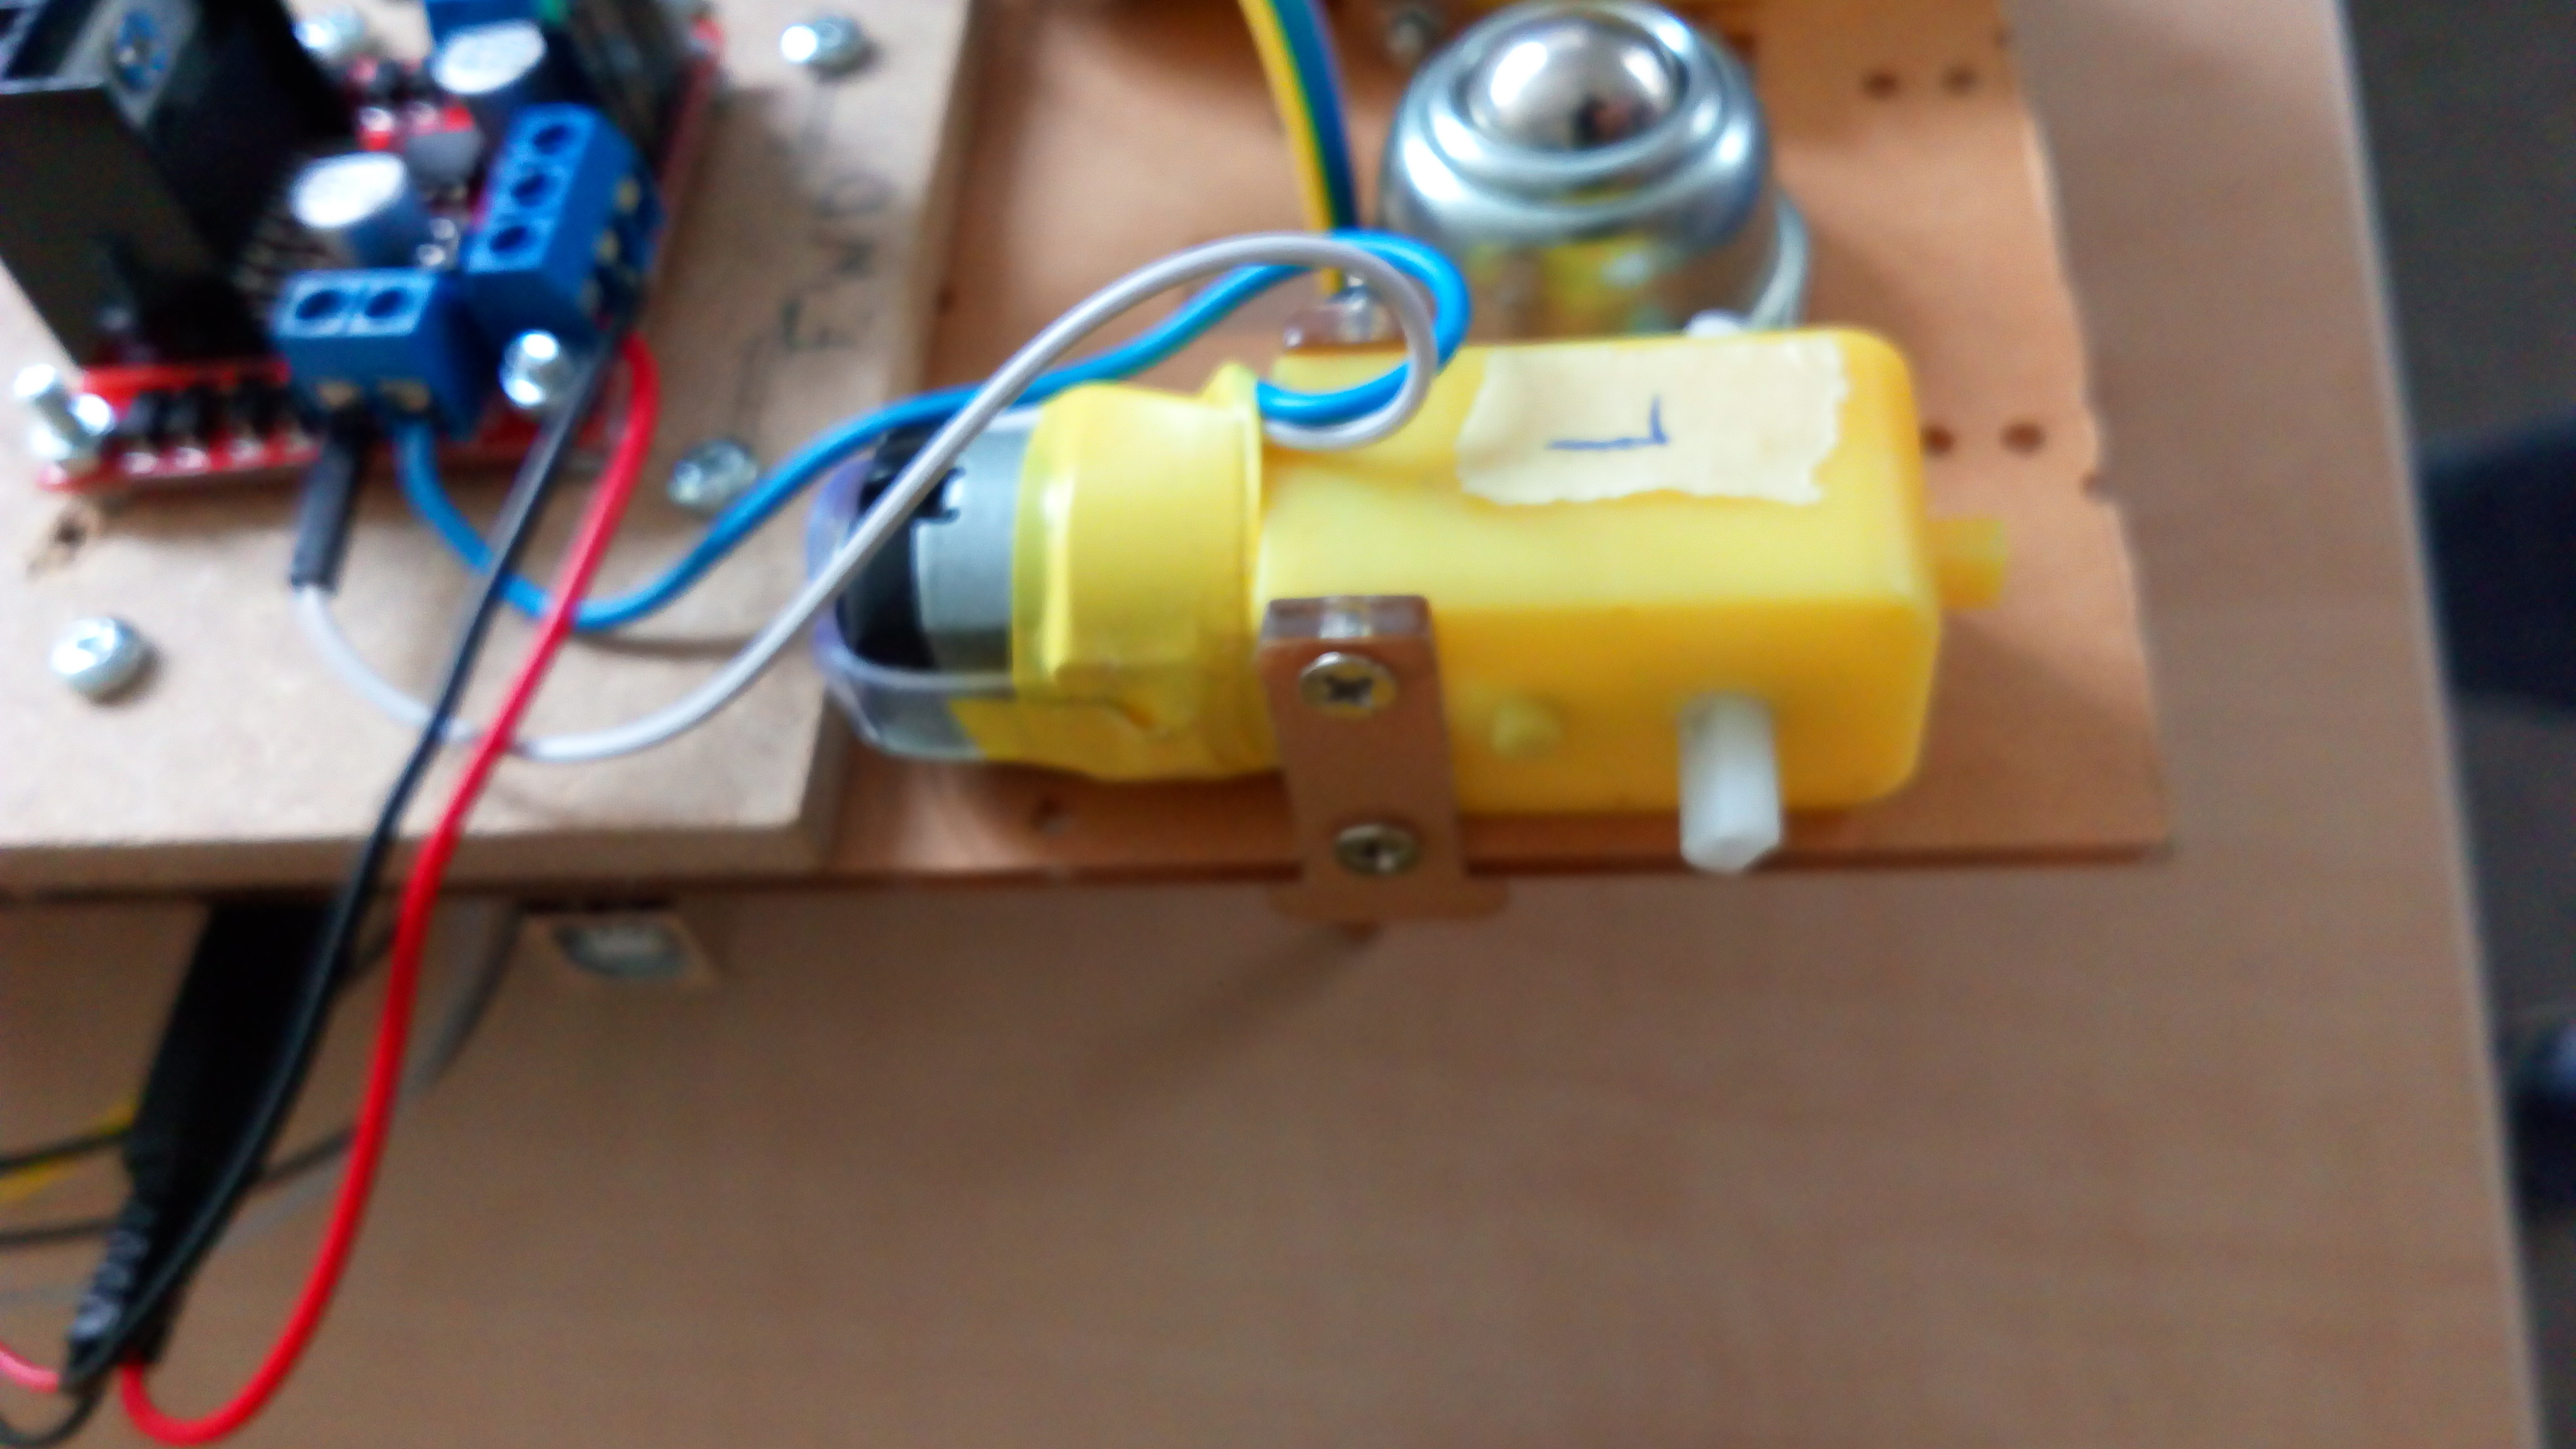
\includegraphics[width=0.7\linewidth]{vastzetten_motor}
		\label{fig:vastzetten_motor}
	\end{figure}
	\item Monteer de plank in de lengte aan het autochasis.
	\begin{figure}[H]
		\centering
		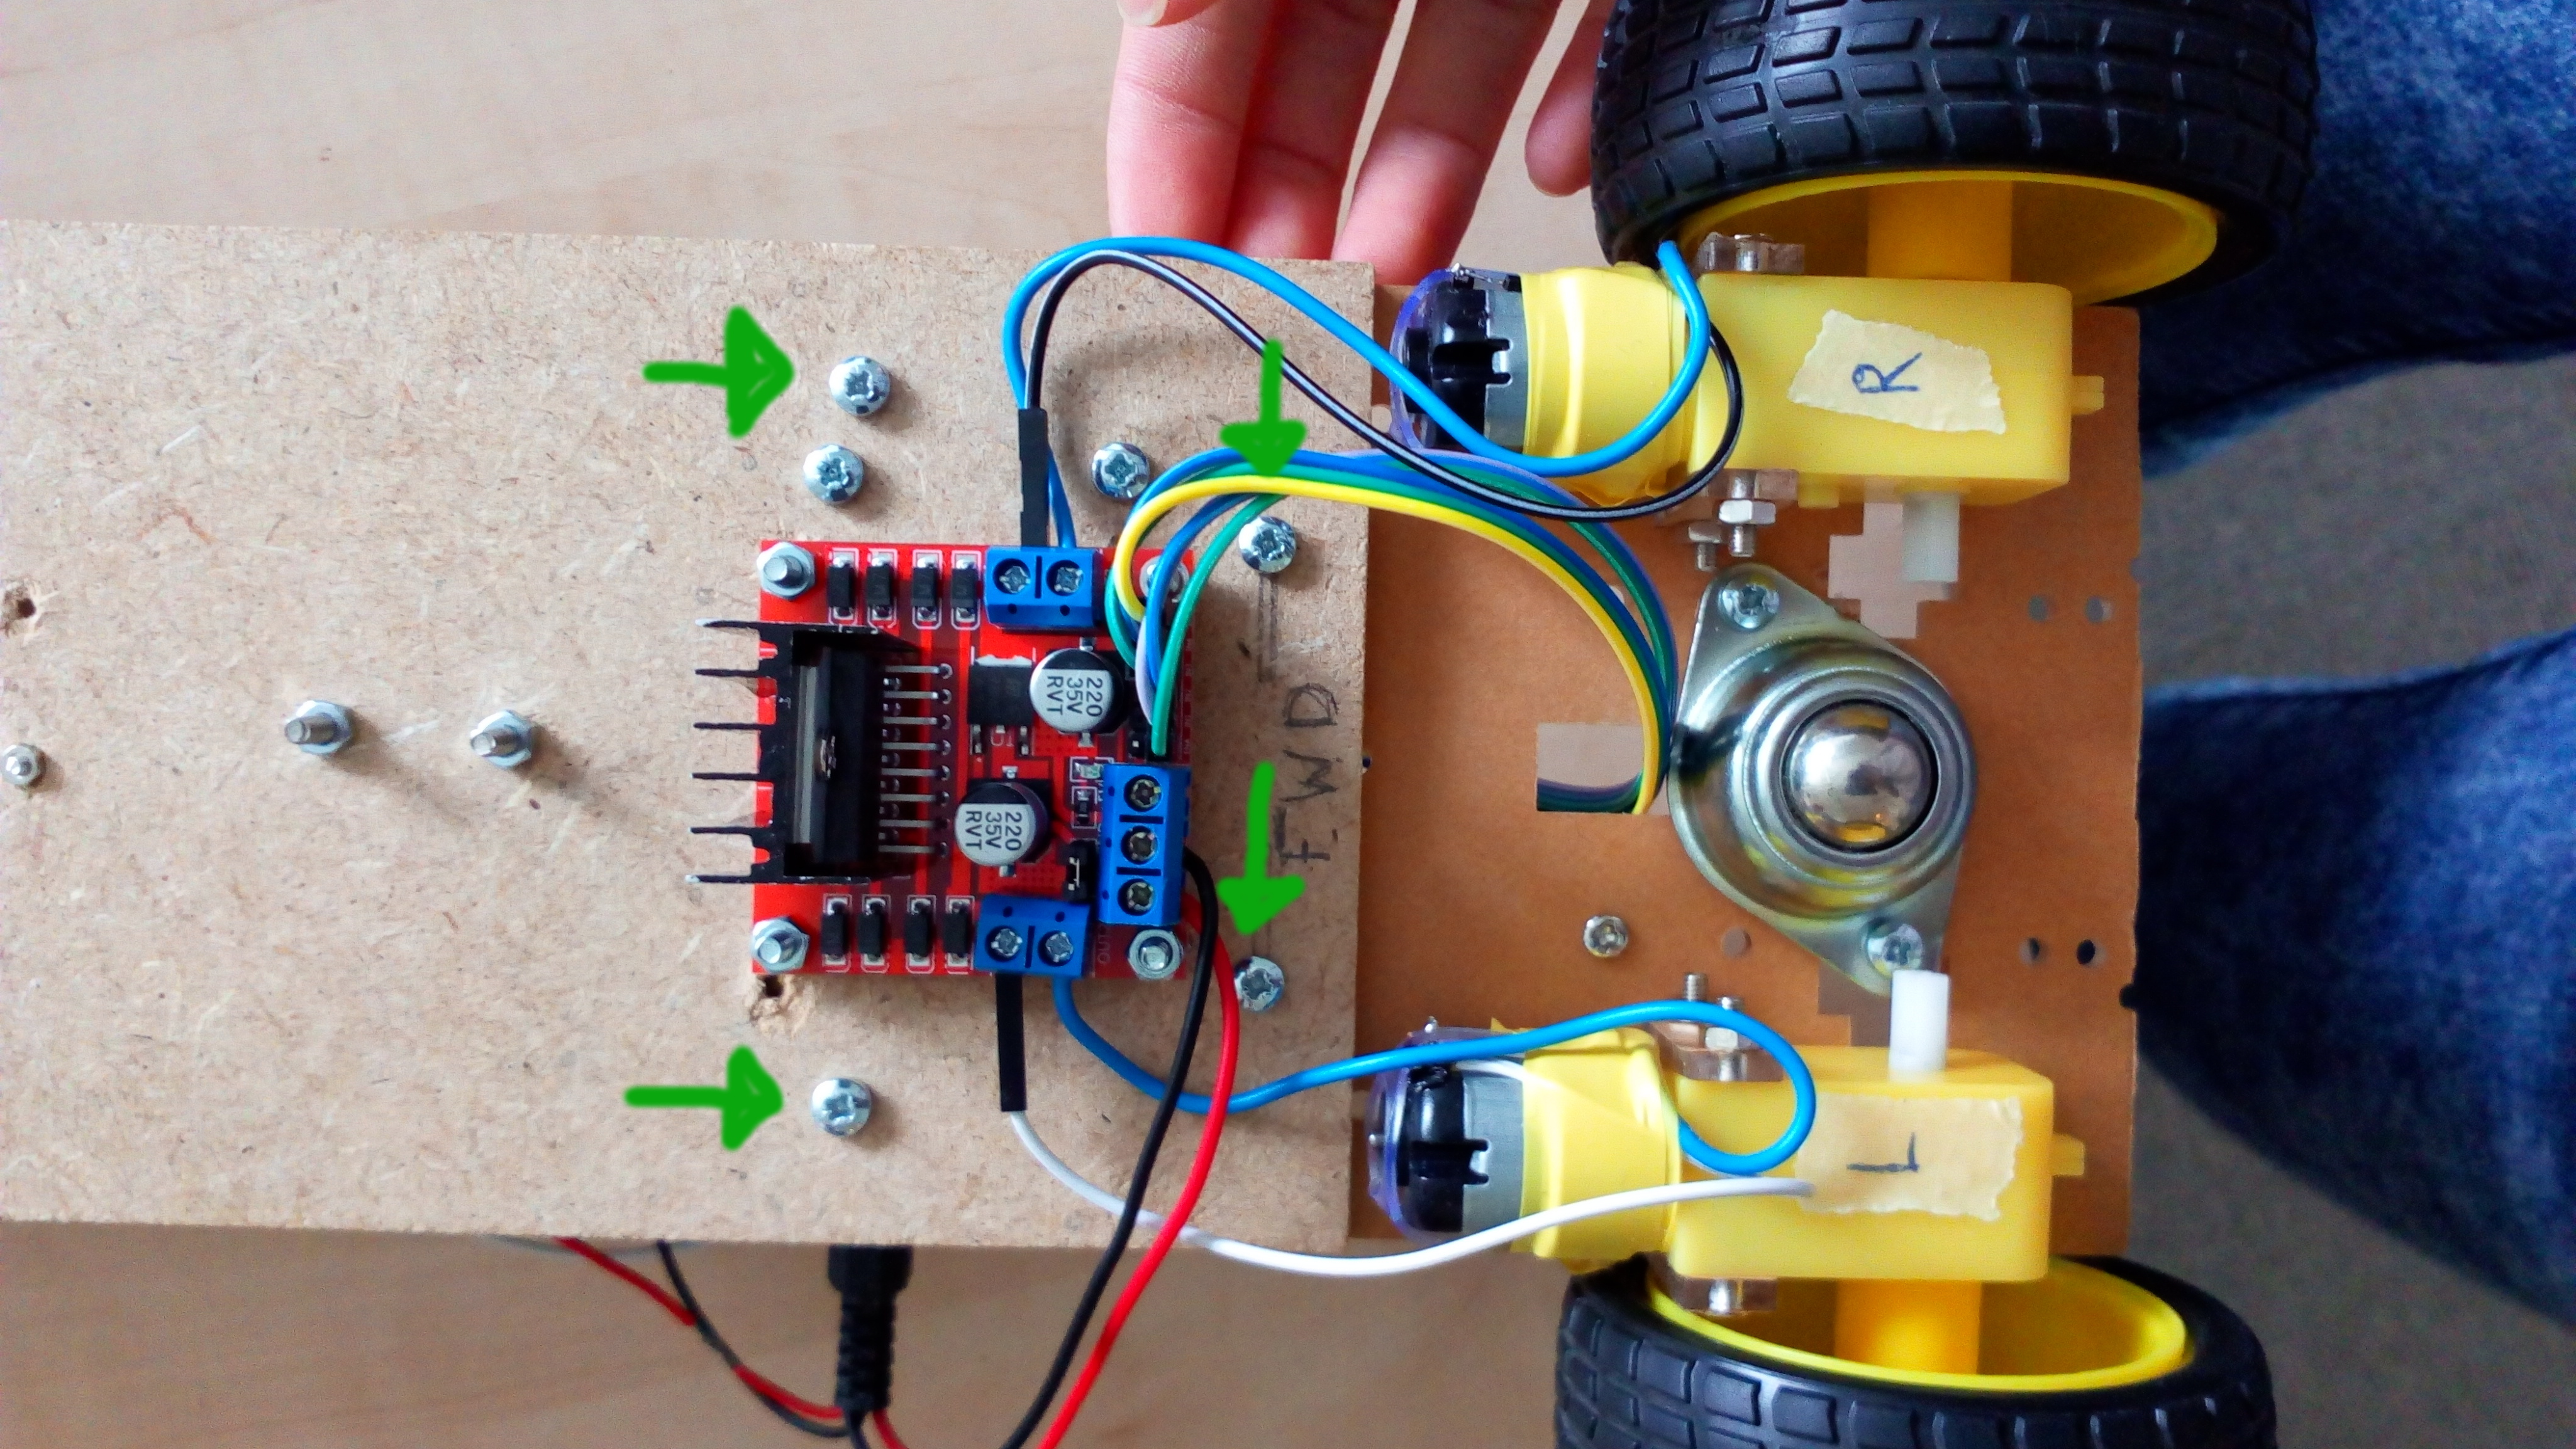
\includegraphics[width=0.7\linewidth]{vastzetten_plank}
		\label{fig:vastzetten_plank}
	\end{figure}
	\item Monteer de motor controller op de plank. 
	\begin{figure}[H]
		\centering
		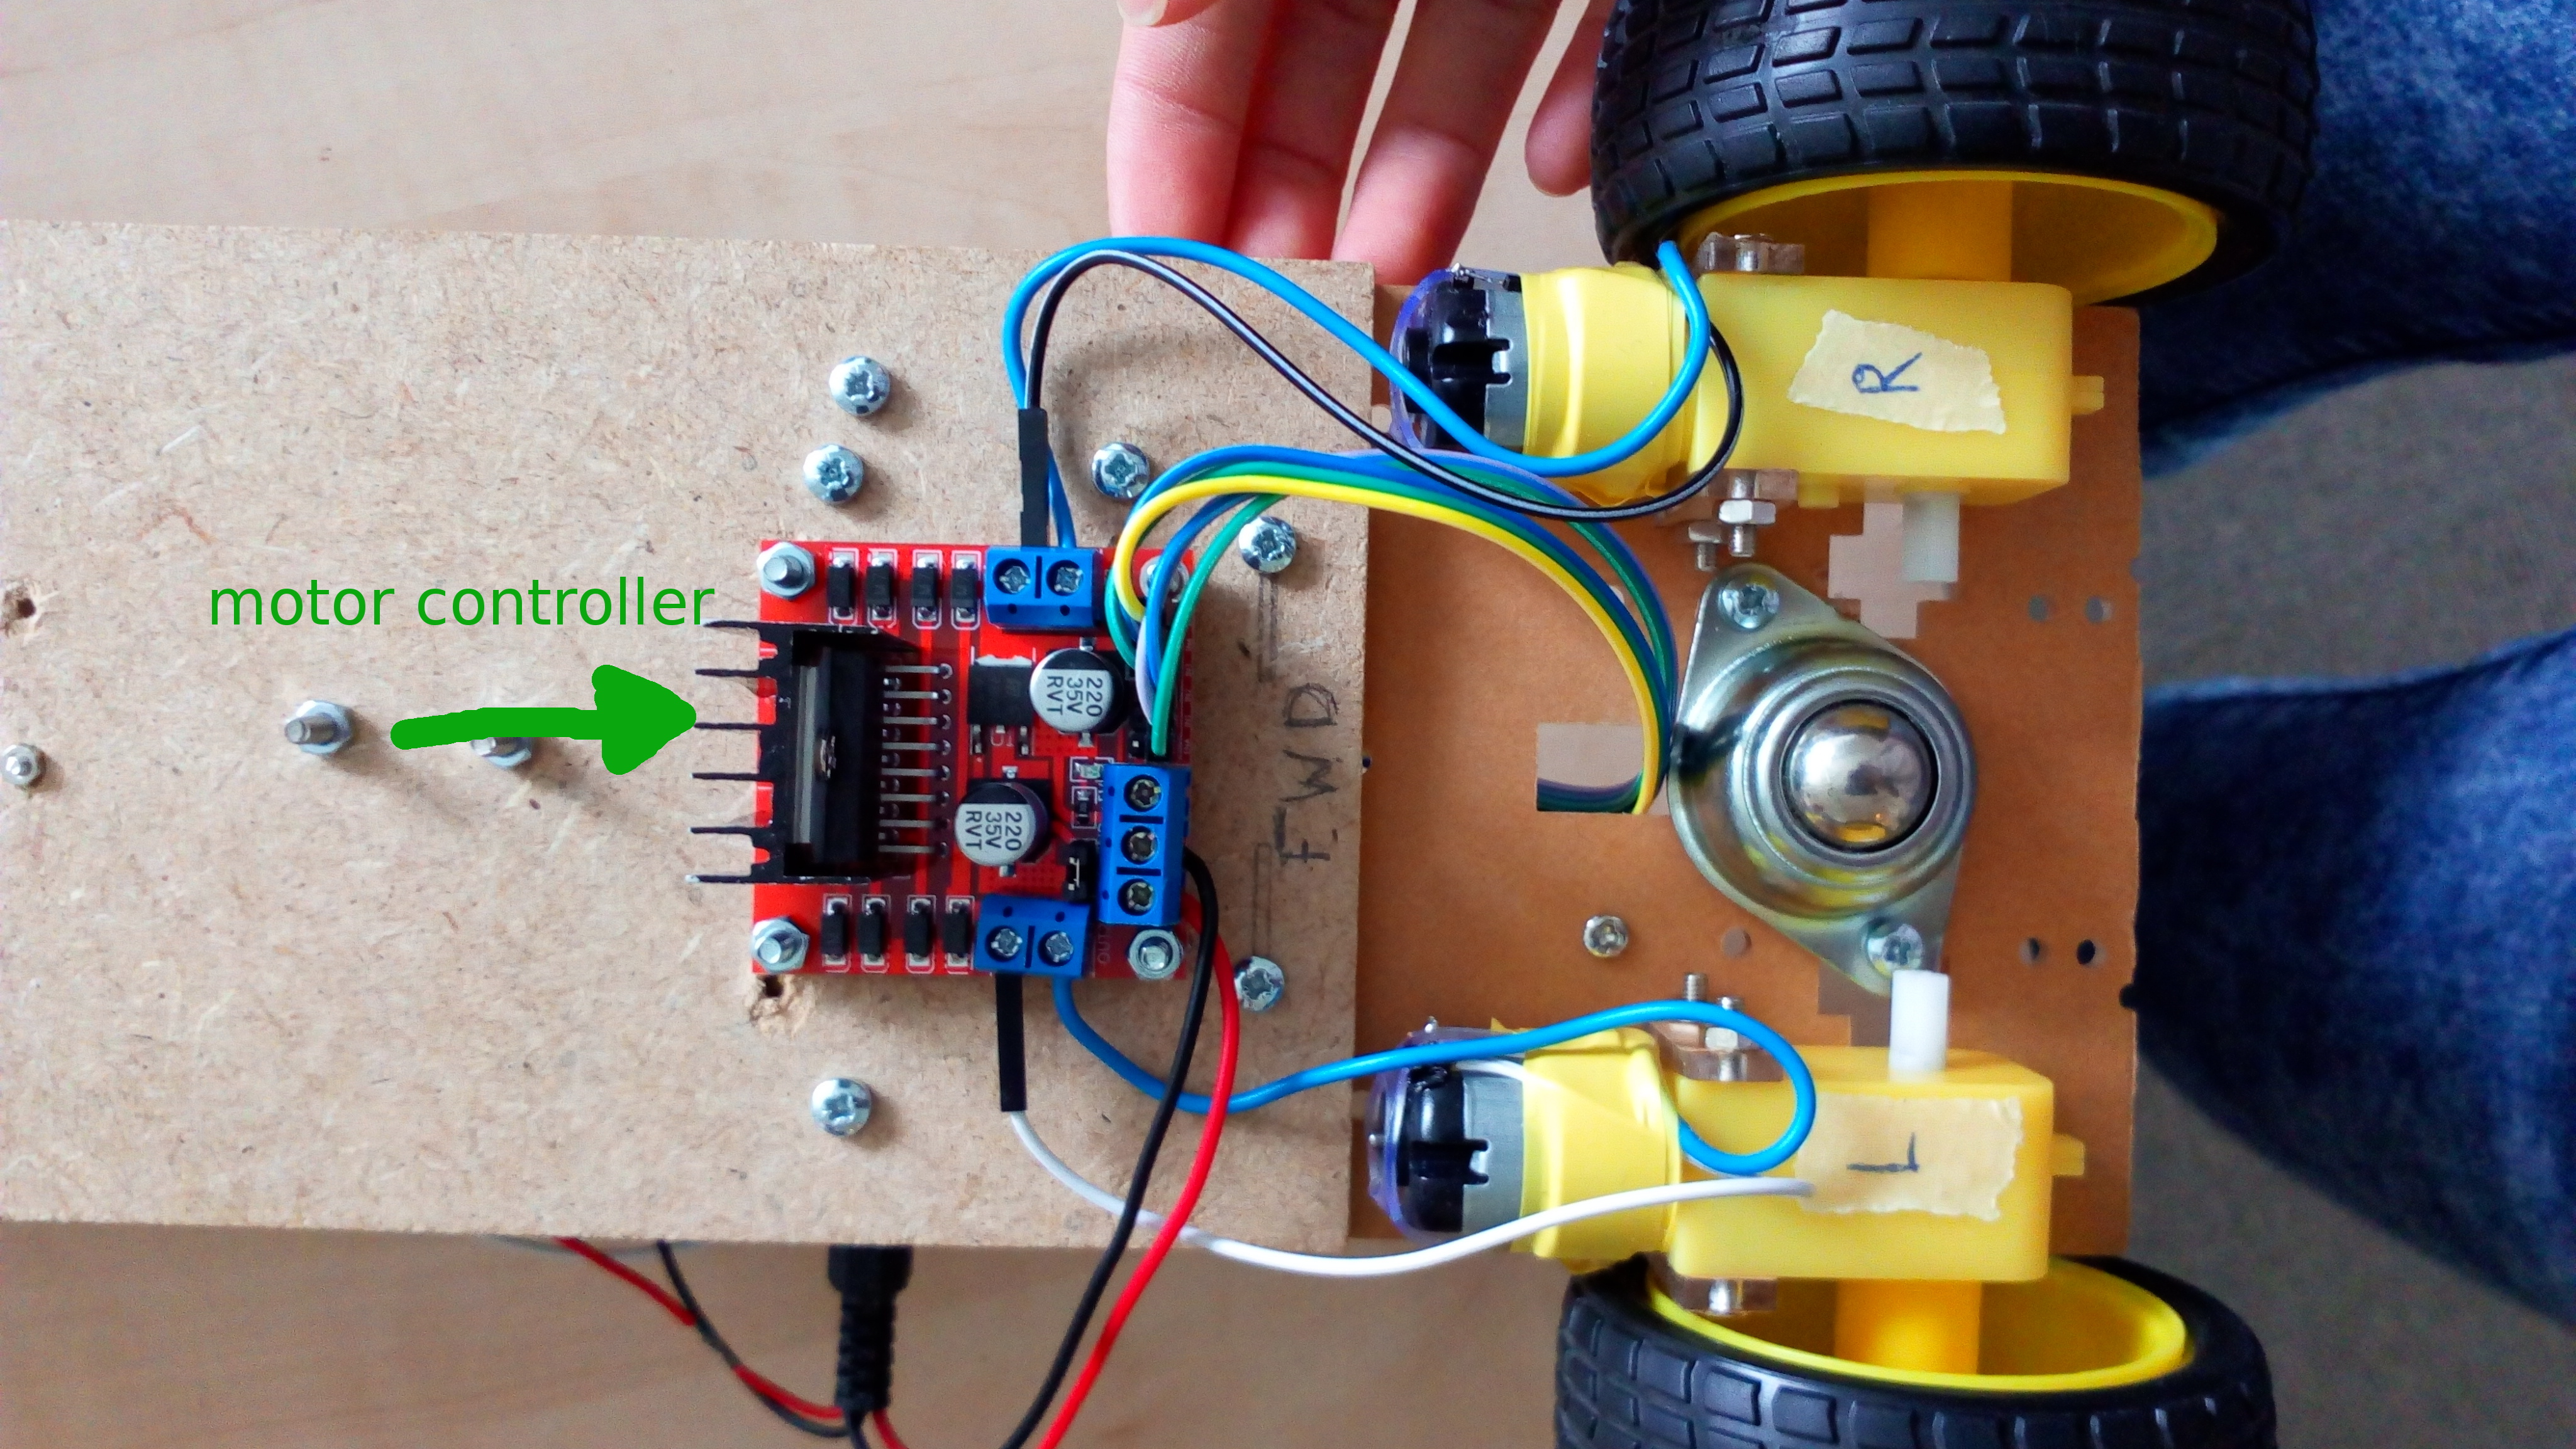
\includegraphics[width=0.7\linewidth]{vastzetten_motorcontroller}
		\label{fig:vastzetten_mc}
	\end{figure}
	\item Monteer de Arduino, batterijhouder en de absolute orientation sensor.
	\begin{figure}[H]
		\centering
		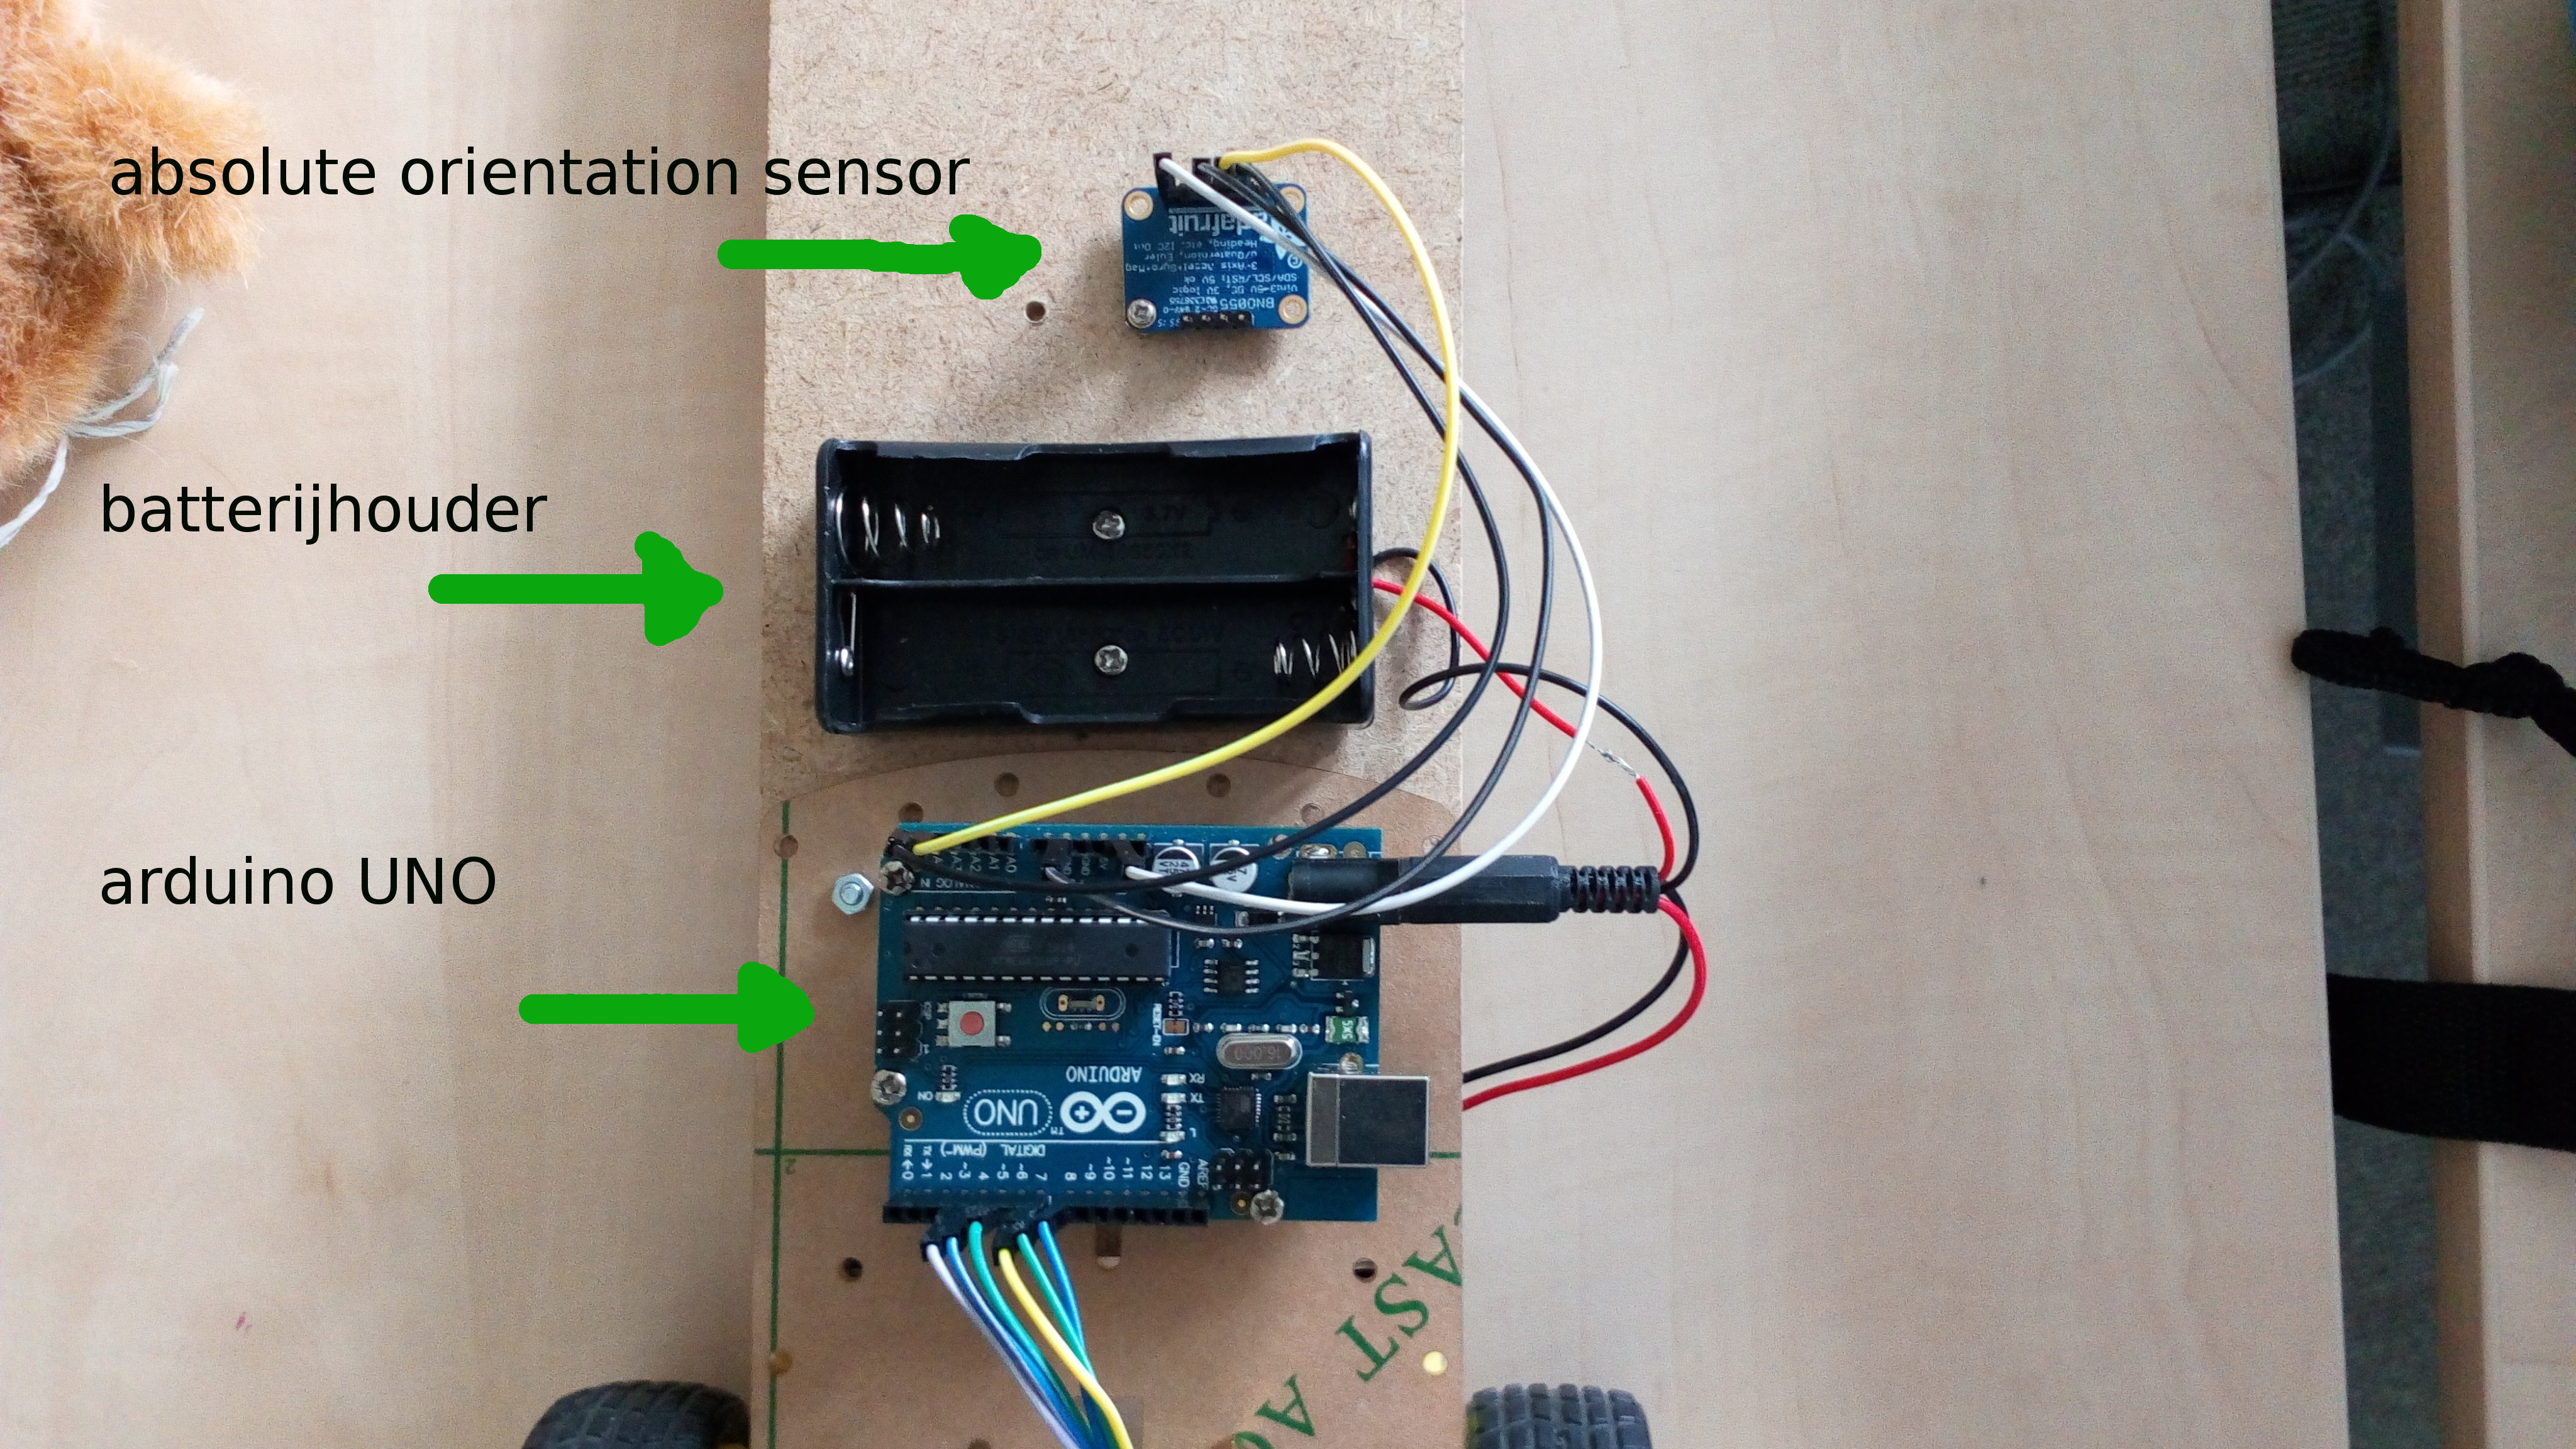
\includegraphics[width=0.7\linewidth]{vastzetten_onderdelen}
		\label{fig:vastzetten_onderdelen}
	\end{figure}
	\begin{figure}[H]
		\centering
		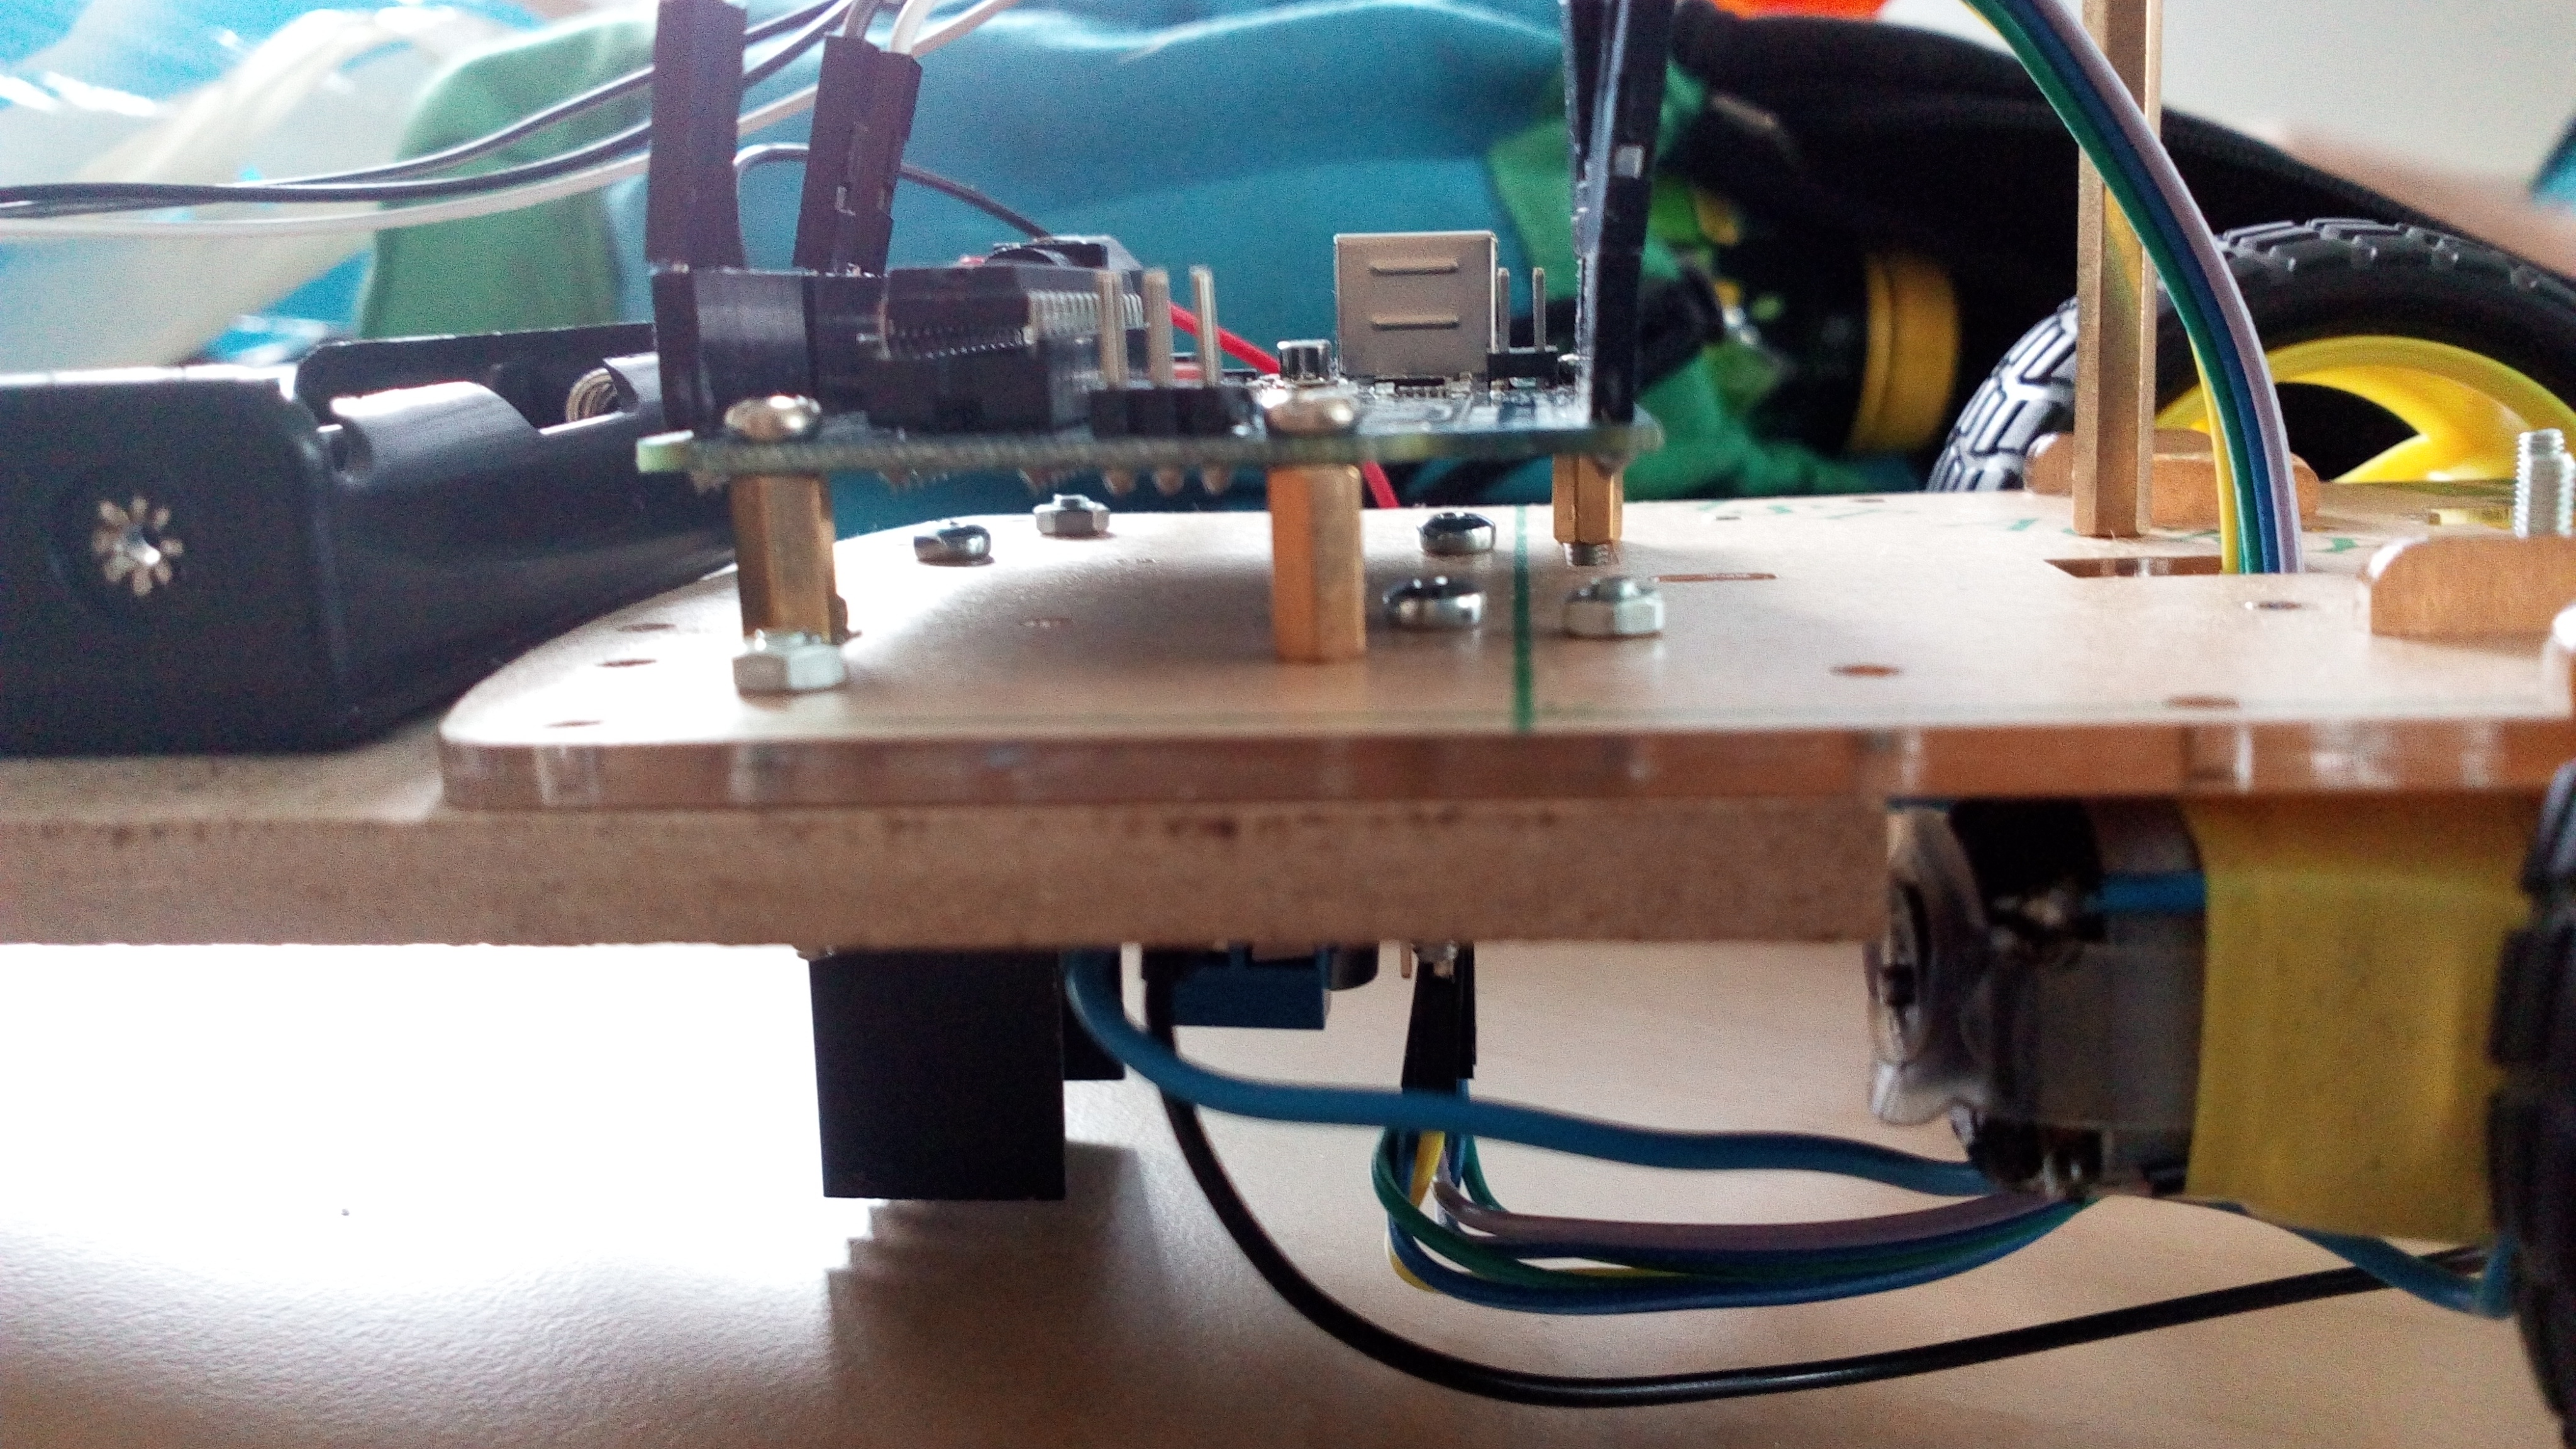
\includegraphics[width=0.7\linewidth]{vastzetten_zijkant}
		\label{fig:vastzetten_zijkant}
	\end{figure}	
\end{enumerate}

\subsubsection{Aansluitingen}
De onderdelen moeten als volgt aangesloten worden:

\begin{figure} [H]
	\begin{tabularx}{\textwidth}{|X|X|}	
		\hline \multicolumn{2}{|c|}{\textbf{Wheelie}}	\\	
		\hline \multicolumn{2}{|c|}{\textbf{adafruit BNO055 (Absolute Orienation Sensor)}}	\\	
		\hline \textbf{Aansluiting op onderdeel} & \textbf{Aansluiting op Arduino} \\ 
		\hline VIN & 3.5V \\ 
		\hline GND & GND\\ 
		\hline SCL & A5 \\  
		\hline SDA & A4 \\
		\hline \multicolumn{2}{|c|}{\textbf{L298N (Dual H-bridge Motor Controller)}}	\\	 
		\hline \textbf{Aansluiting op onderdeel} & \textbf{Aansluiting op Arduino} \\
		\hline GND & GND \\
		\hline ENA & 5  \\
		\hline ENB & 6 \\
		\hline IN1 & 3 \\
		\hline IN2 & 4 \\
		\hline IN3 & 7 \\
		\hline IN4 & 8 \\
		\hline \textbf{Aansluiting op onderdeel} & \textbf{Aansluiting op motor L} \\
		\hline OUT1 & witte draad \\
		\hline OUT2 & blauwe draad \\
		\hline \textbf{Aansluiting op onderdeel} & \textbf{Aansluiting op motor R} \\
		\hline OUT3 & blauwe draad \\
		\hline OUT4 & zwarte draad \\
		\hline \multicolumn{2}{|c|}{\textbf{Batterijhouder}}\\	 
		\hline \textbf{Aansluiting op onderdeel} & \textbf{Aansluiting op Arduino} \\
		\hline grote ronde stekker & DC input \\
		\hline \textbf{Aansluiting op onderdeel} & \textbf{Aansluiting op motor controller} \\
		\hline zwarte draad & GND \\
		\hline rode draad & 12V \\		
		\hline		
	\end{tabularx} 
	\caption{Aansluitingen Wheelie}
	\label{tbl:Aansluitingen_Wheelie}
\end{figure}

\newpage
\subsection{Auto}
\subsubsection{Onderdelen}
Auto is gebaseerd op de Bluetooth Controlled Robot Car Kits for Arduino \cite{DIY_auto}. Voor Auto zijn de volgende onderdelen nodig. 

\begin{table}[!h]	
	\begin{tabular}{|l|c|}
		\hline \multicolumn{2}{|c|}{\textbf{Auto}}	\\	
		\hline \textbf{Onderdelen} & \textbf{Aantal} \\ 
		\hline Arduino LEONARDO & 1 \\ 
		\hline  nRF8001 (Bluetooth LE) & 1  \\ 
		\hline	L298 (Dual H-bridge Motor Controller) & 1 \\
		\hline Ai-Ball & 1 \\
		\hline  CR2 batterij & 1 \\
		\hline  batterijhouder & 1  \\ 
		\hline 3400 mAh 3.6V batterij & 2 \\ 
		\hline  geared motor & 4 \\
		\hline  wiel	 & 4 \\
		\hline 	100 x 213 x 5mm acrylic glass plate (bxlxh) & 2 \\
		\hline  motor fixing & 4 \\
		\hline	koper pilaar 40 mm (l) & 6 \\
		\hline 	koper pilaar 10 mm (l) & 2 \\
		\hline 	schroeven 3x20 mm (dxl) & - \\
		\hline	schroeven 3x12 mm (dxl) & - \\
		\hline  moeren M3 & - \\	
		\hline
	\end{tabular} 
	\caption{Onderdelen Auto}
	\label{tbl:Onderdelen_auto}
\end{table}
	
\subsubsection{Montage}
Voor de montage van Auto kun je voor het grootste gedeelte gelijk aan die van de robot-car.

\begin{enumerate}
	\item Monteer alle onderdelen hierboven \ref{tbl:Onderdelen_auto} zoals in de handleiding is aangegeven \cite{DIY_auto_hl}. 
	\item Monteer de nRF8001 (Bluetooth LE).
	\begin{figure}[H]
	\centering
	\includegraphics[width=0.7\linewidth]{vastzetten_auto}
	\label{fig:vastzetten_auto}
	\end{figure}
	\begin{figure}[H]
		\centering
		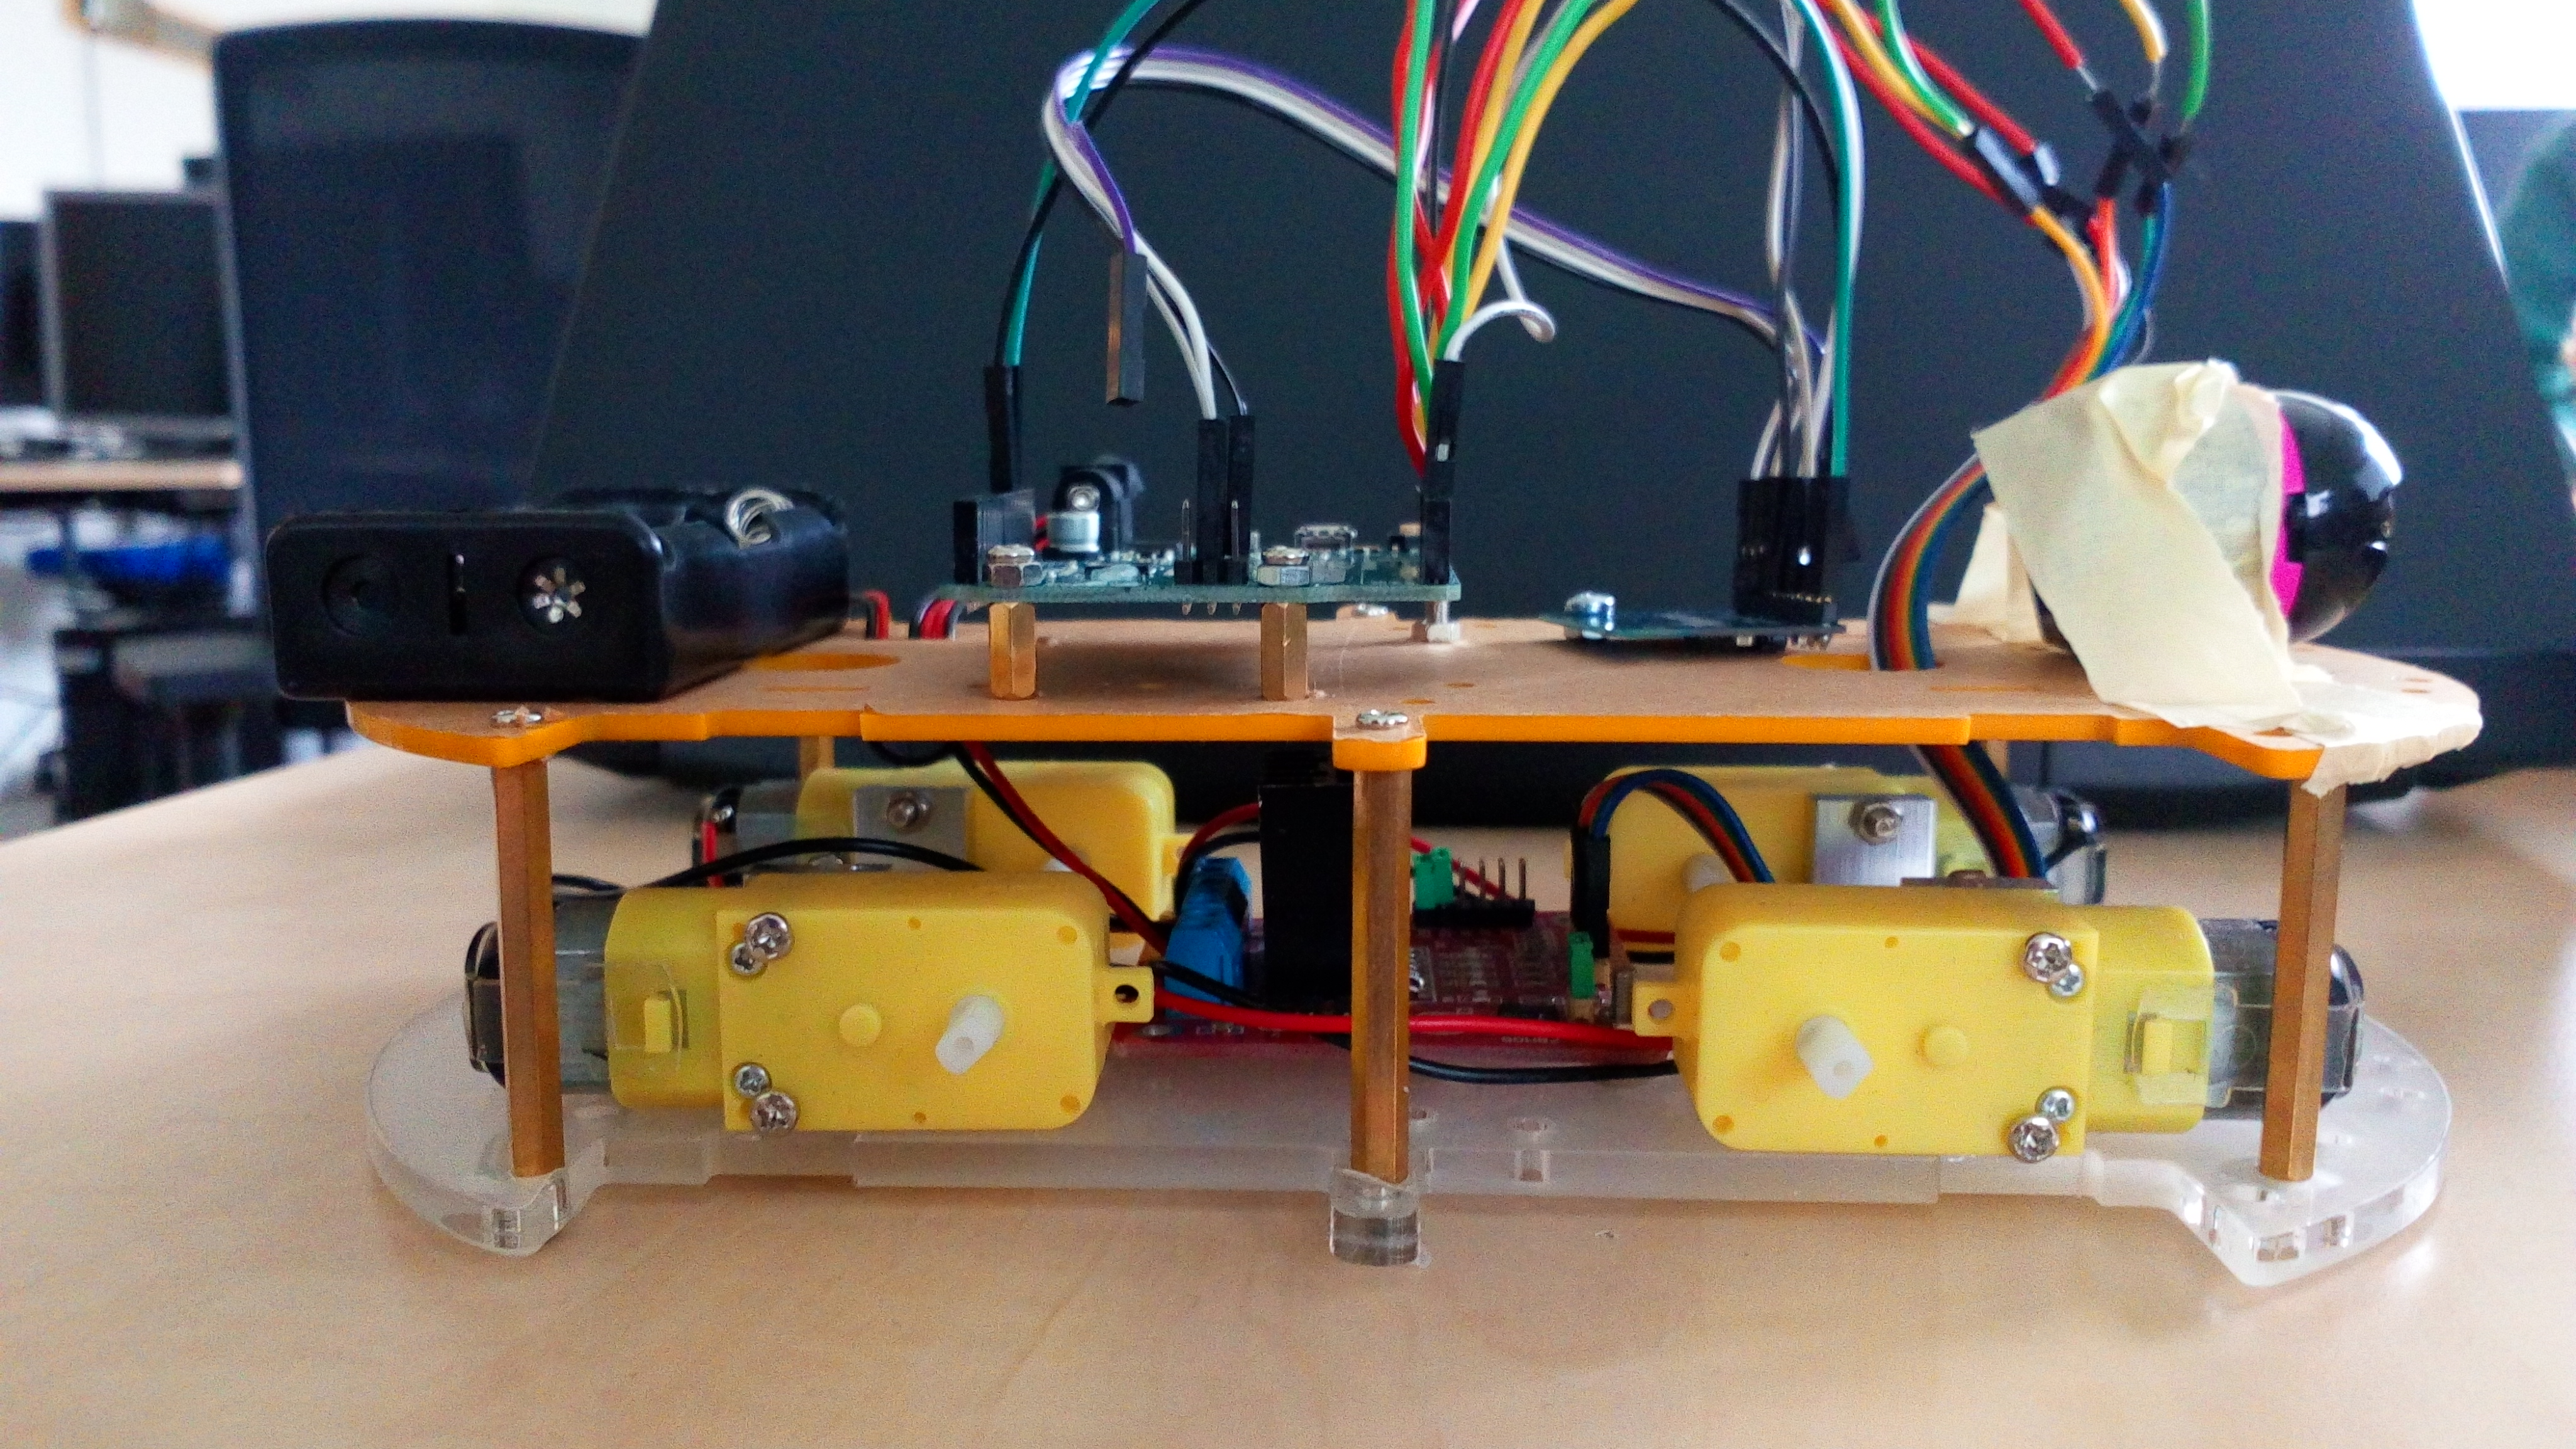
\includegraphics[width=0.7\linewidth]{zijkant}
		\label{fig:vastzetten_zijkant_auto}
	\end{figure}
	\item Monteer de Ai ball.
	\begin{figure}[H]
		\centering
		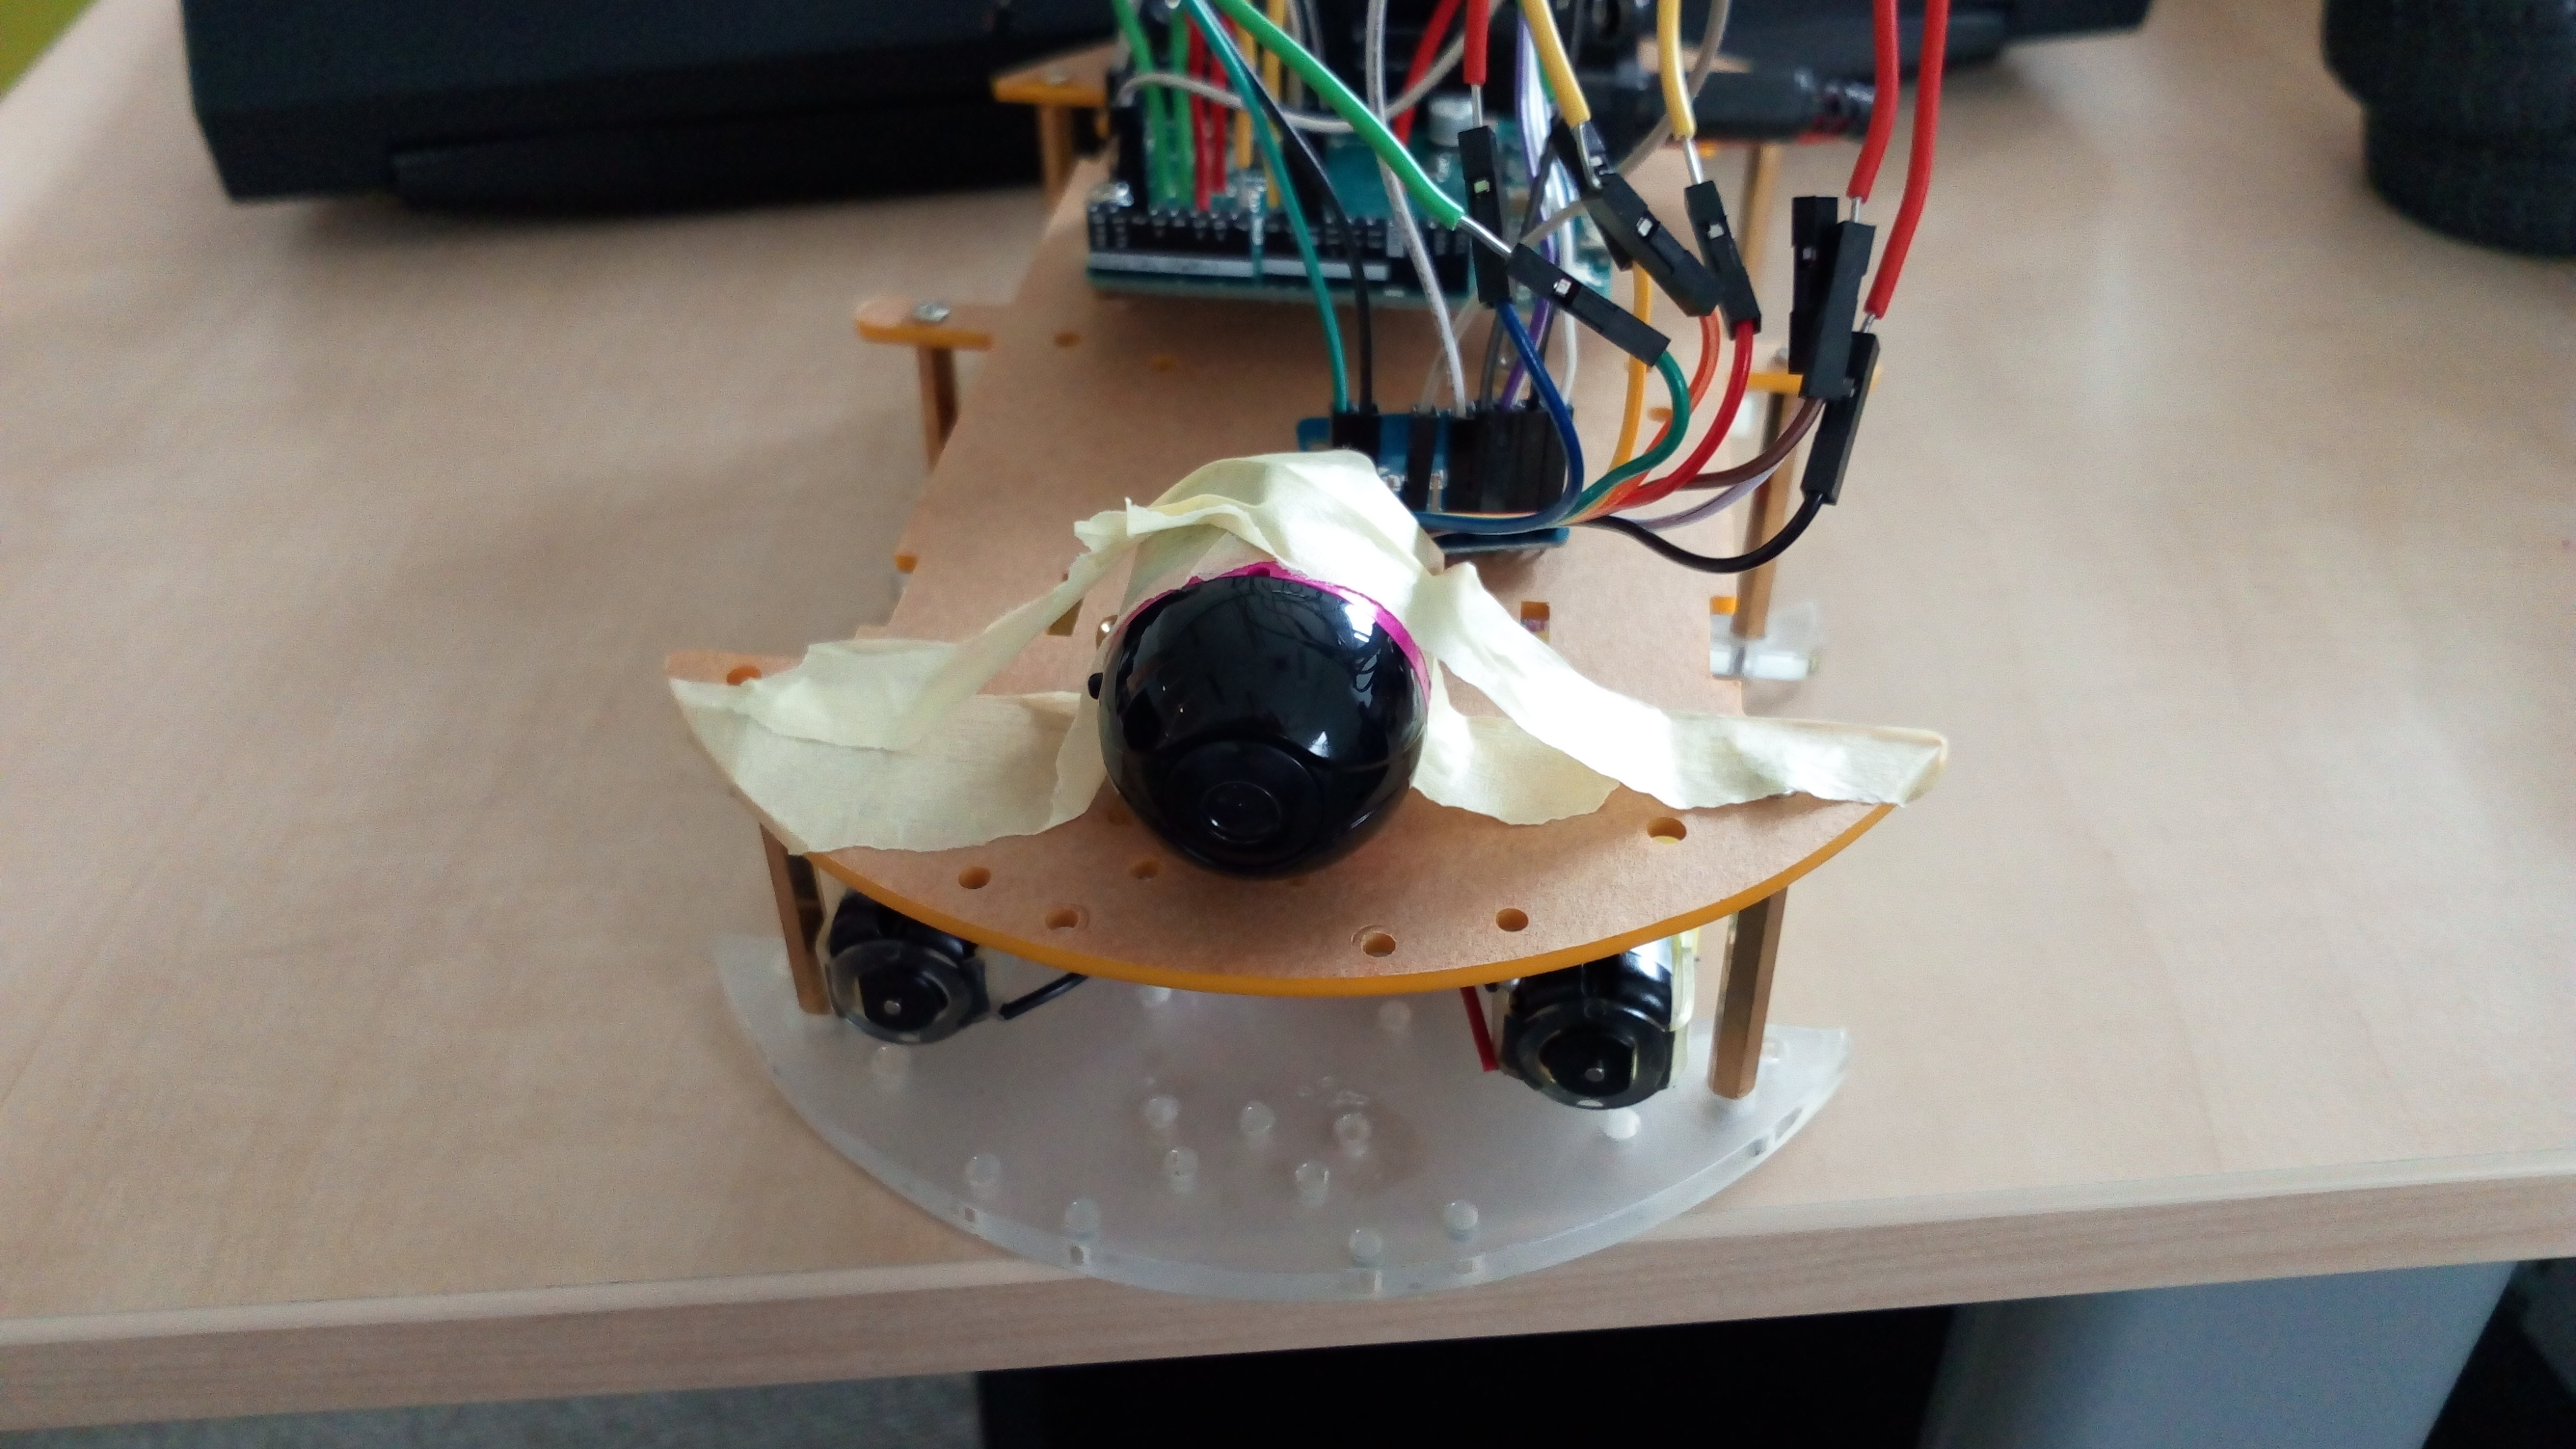
\includegraphics[width=0.7\linewidth]{ai_ball}
		\label{fig:vastzetten_aiball}
	\end{figure}	
\end{enumerate}
	
\newpage
\subsubsection{Aansluitingen}
De onderdelen worden als volgt aangesloten.			
\begin{table}[H]
	\begin{tabularx}{\textwidth}{|X|X|}	
		\hline \multicolumn{2}{|c|}{\textbf{nRF8001 (Bluetooth LE)}}	\\	 
		\hline \textbf{Aansluiting op onderdeel} & \textbf{Aansluiting op Arduino} \\
		\hline VIN & 5v \\
		\hline GND & GND \\
		\hline SCK &  ICSP 3 (ICSP links-midden)\\
		\hline MISO & ICSP 1 (ICSP links-boven)\\
		\hline MOSI & ICSP 4 (ICSP rechts-midden)\\
		\hline REQ & 10 \\
		\hline RST & 9 \\
		\hline RDY & 2 \\
		\hline \multicolumn{2}{|c|}{\textbf{L298 (Dual H-bridge Motor Controller)}}	\\	 
		\hline \textbf{Aansluiting op onderdeel} & \textbf{Aansluiting op Arduino} \\
		\hline GND & GND \\
		\hline ENA & 5  \\
		\hline ENB & 6 \\
		\hline IN1 & 3 \\
		\hline IN2 & 4 \\
		\hline IN3 & 7 \\
		\hline IN4 & 8 \\
		\hline \textbf{Aansluiting op onderdeel} & \textbf{Aansluiting op motor LV} \\
		\hline OUT1 & rode draad \\
		\hline OUT2 & zwarte draad \\
		\hline \textbf{Aansluiting op onderdeel} & \textbf{Aansluiting op motor LA} \\
		\hline OUT1 & rode draad \\
		\hline OUT2 & zwarte draad \\
		\hline \textbf{Aansluiting op onderdeel} & \textbf{Aansluiting op motor RV} \\
		\hline OUT3 & zwarte draad \\
		\hline OUT4 & rode draad \\
		\hline \textbf{Aansluiting op onderdeel} & \textbf{Aansluiting op motor RA} \\
		\hline OUT3 & zwarte draad \\
		\hline OUT4 & rode draad \\
		\hline \multicolumn{2}{|c|}{\textbf{Batterijhouder}}\\	 
		\hline \textbf{Aansluiting op onderdeel} & \textbf{Aansluiting op Arduino} \\
		\hline grote ronde stekker & DC input \\
		\hline \textbf{Aansluiting op onderdeel} & \textbf{Aansluiting op motor controller} \\
		\hline zwarte draad & GND \\
		\hline rode draad & 12V \\		
		\hline		
	\end{tabularx} 
	\caption{Aansluitingen Auto}
	\label{tbl:Aansluitingen_auto}
\end{table}

\section{Software}
Alle software voor dit project staat als zipbestand op de New devices lab wiki. De code is ook te downloaden van github.
\url{https://github.com/Lucus16/NDL/}

\subsection{Arduino}
Voor dit project is gebruik gemaakt van de Arduino IDE ARDUINO (ARDUINO 1.6.7). De laatste versie van ARDUINO is te downloaden op onderstaande link: \url{https://www.arduino.cc/en/Main/Software}. Deze software is beschrikbaar voor Windows, Mac OS X en Linux. Op de website van Arduino staan ook instructies voor het installeren van de IDE en verdere documentatie \cite{ARDUINO_getting started}.

Hieronder vind je een tabel met alle gebruikte libraries voor dit project.
Eerst komen alle libraries die gebruikt zijn in de code voor de arduino's.

\begin{table}[H]
	\begin{tabularx}{\textwidth}{|l|l|X|}
		%\hline \textbf{Bibliotheek} & \textbf{Versie} & \textbf{Download link}  \\ 
		%\hline Wire & 1.0 & - \\ 
		%\hline SPI & 1.0 & - \\ 
		%\hline SoftwareSerial & 1.0 & - \\ 
		%\hline Adafruit\_Sensor & 1.0.2 &  \url{https://github.com/adafruit/Adafruit_Sensor/archive/master.zip}  \\ 
		\hline Adafruit\_BNO055 & 1.1.2 & \url{https://github.com/adafruit/Adafruit_BNO055/archive/master.zip} \\ 
		\hline Adafruit\_BLE\_UART & 1.0.0 & \url{https://github.com/adafruit/Adafruit_nRF8001/archive/master.zip }\\ 
		\hline		
	\end{tabularx} 
	\caption{Arduino libraries Wheelie}
	\label{tbl:Download_link}
\end{table}
\begin{table}[H]
	\begin{tabularx}{\textwidth}{|l|l|X|}
		%\hline \textbf{Bibliotheek} & \textbf{Versie} & \textbf{Download link}  \\ 
		%\hline Wire & 1.0 & - \\ 
		%\hline SPI & 1.0 & - \\ 
		%\hline SoftwareSerial & 1.0 & - \\ 
		%\hline Adafruit\_Sensor & 1.0.2 &  \url{https://github.com/adafruit/Adafruit_Sensor/archive/master.zip}  \\ 
		%\hline Adafruit\_BNO055 & 1.1.2 & \url{https://github.com/adafruit/Adafruit_BNO055/archive/master.zip} \\ 
		\hline Adafruit\_BLE\_UART & 1.0.0 & \url{https://github.com/adafruit/Adafruit_nRF8001/archive/master.zip }\\ 
		\hline		
	\end{tabularx} 
	\caption{Arduino libraries Auto}
	\label{tbl:Download_link auto}
\end{table}

Deze libraries moeten handmatig toegevoegd worden. De download links in Tabel \ref{tbl:Download_link} verwijzen naar een .zip bestand met de gewenste library. De libraries kun je aan de Arduino IDE toevoegen door in het menu van de IDE te klikken op $$ \text{Sketch} \rightarrow \text{Include Library }\rightarrow \text{Add .ZIP Library ..}$$ en hier de gewenste .zip bestand te selecteren.
\begin{figure}[h]
\centering
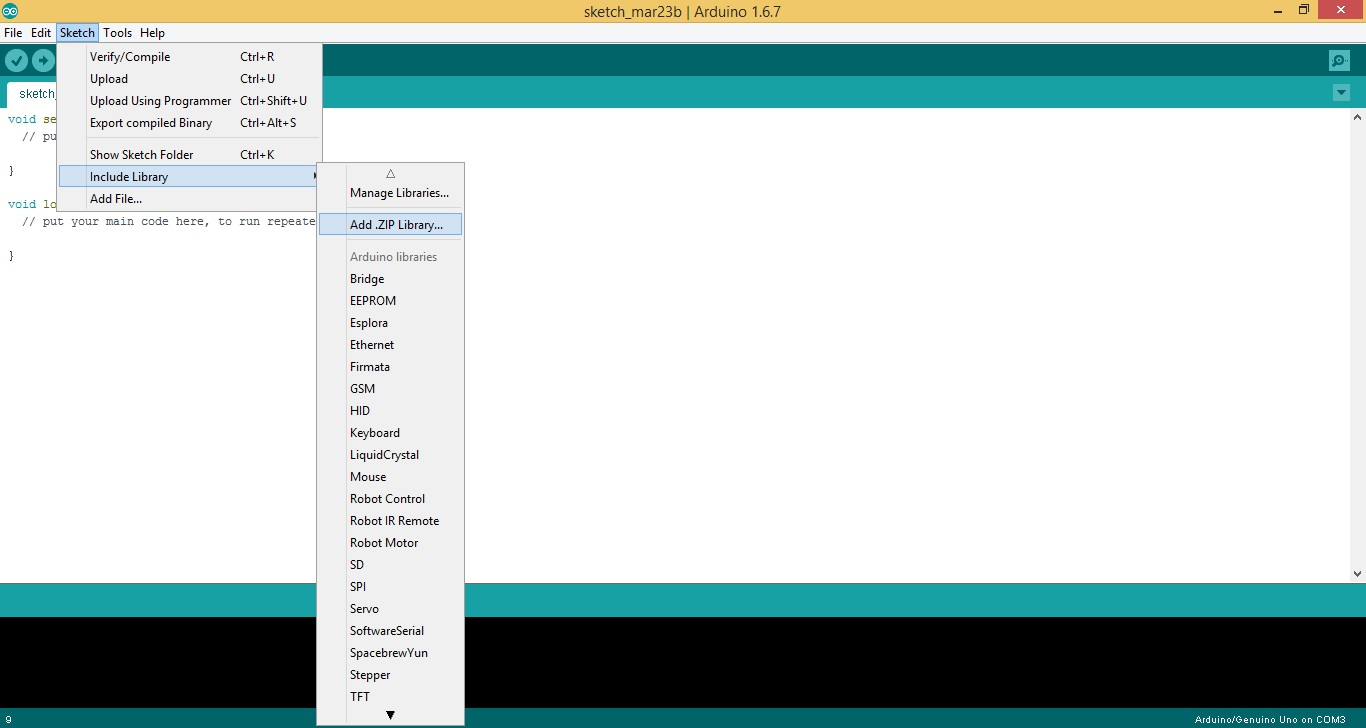
\includegraphics[width=0.7\linewidth]{Add_ZIP}
\label{fig:Add_ZIP}
\end{figure}

\newpage
Om de code op de arduino te zetten moet je de volgende stappen doen:
\begin{enumerate}
	\item Verbind de Arduino met de computer via de bijgeleverde USB-kabel.
	\item Open de code die je op de Arduino wilt zetten.
		\begin{enumerate}
			\item Wheelie.ino voor Wheelie.
			\item Auto.ino voor Auto.
		\end{enumerate}
	\item Kies de juiste Arduino versie.  
	\begin{enumerate}
		\item $ \text{Tools} \rightarrow \text{Board} \rightarrow \text{Arduino/Genuino Uno} $ voor Wheelie.
		\item $ \text{Tools} \rightarrow \text{Board} \rightarrow \text{Arduino/Genuino Leonardo} $ voor Auto.
	\end{enumerate}	
	\begin{figure}[h]
		\centering
		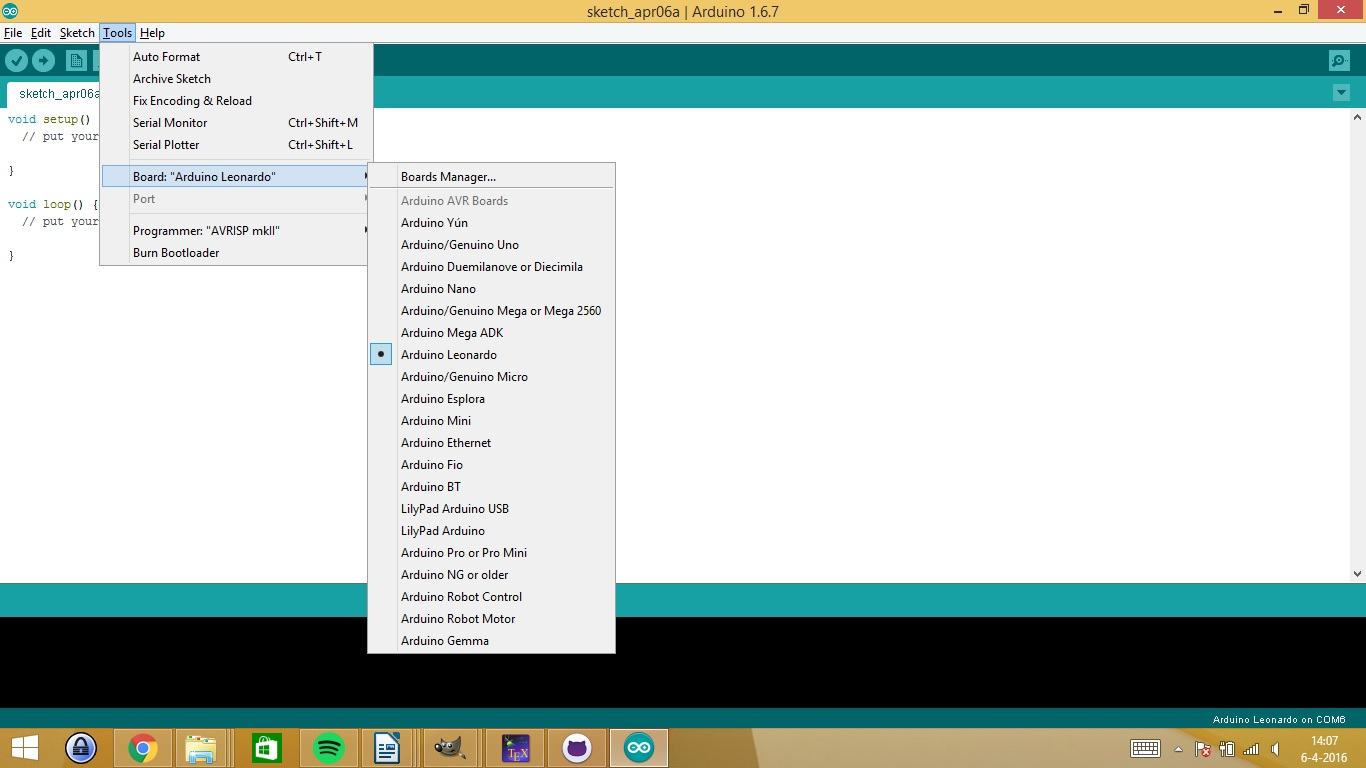
\includegraphics[width=0.7\linewidth]{board_selecteren}
		\label{fig:board_selecteren}
	\end{figure}
	\item Upload de code naar de Arduino.		
\end{enumerate}

\subsection{Android}
Voor deze app hebben we de code van de open-source nrF-UART implementatie \cite{nrf_ua} gebruikt als basis voor onze eigen app. 
De app draait op android 4.3 en hoger en is te installeren met iedere android IDE. 

\section{Gebruik}
In dit hoofdstuk staat beschreven hoe je Wheelie en Auto daadwerkelijk kunt gebruiken. Als eerste komt Wheelie aan bod, gevolgd door Auto.

\subsection{Wheelie}
Wheelie is als volgt te gebruiken:
	
\begin{enumerate}
	\item Doe de batterijen in de batterijhouder.
	\item Zet de Wheelie rechtop (verticaal) op de grond. 
	Na een paar seconden kun je Wheelie loslaten. Hierna zal de robot zichzelf balanceren door voor en achteruit te rijden. 
	\item Blijf in de buurt om Wheelie op te vangen.
	De huidige code werkt nog niet perfect. Daardoor is het nodig om naast Wheelie te blijven staan om hem op te vangen als hij valt. Aan beide kanten van de robot zitten uitsteeksels waardoor de hardware niet snel zal beschadigen bij een val, maar voorkoming is altijd beter. 
	\item Verbind Wheelie met de android app. 
	Dit doe je door de instructies onder \"4.4 android app\" te volgen.
	\item Bestuur Wheelie met je mobiel.
	Het idee achter de besturing is dat Wheelie de positie van je mobiel nadoet. Zolang je je mobiel verticaal houdt, zal Wheelie stil blijven staan. Als je je mobieltje naar voren kantelt, gaat Wheelie naar voren. Kantel je je mobiel naar achter, zal Wheelie ook naar achter gaan. De richting waar je mobiel kijkt is ook de richting waar Wheelie naar kijkt. Dus als jij een kwartslag draait zal Wheelie hetzelfde doen.
\end{enumerate}

Als Wheelie een hoek van meer dan 45 graden maakt ten opzichte van rechtop staan, zullen de motoren uitgaan. Hierdoor zal hij niet doorrijden als hij al gevallen is. Dit zorgt er ook voor dat je hem horizontaal op tafel kunt leggen zonder dat hij gaat rijden. 

Momenteel is de enige manier om Wheelie uit te zetten de batterijen te verwijderen. Dit kan aangepast worden door een schakelaar aan de batterijhouder te solderen.

Wheelie is ook te besturen met de bijgeleverde app. Hiervoor is het nodig om de bluetooth module te monteren. De Ai-ball kan ook toegevoegd worden voor beeld, maar het werkt ook zonder. Volg de instructies onder het kopje "android app" om Wheelie met de app te verbinden. Hierna kun je Wheelie met je telefoon besturen. 

\subsection{Auto}
Auto is als volgt te gebruiken:

\begin{enumerate}
	\item Doe de batterijen in de batterijhouder.
	\item Verbind Auto met de android app. Dit doe via de instructies onder "android app".
	\item Bestuur Auto met je mobiel. 
	De besturing van Auto lijkt op die van Wheelie. Door je mobiel verder naar voren te kantelen ga je vooruit, door hem naar achter te kantelen ga je achteruit. Voor deze versie van de app hebben we 45 graden als neutrale positie gekozen. Dit hebben we gedaan zodat je ook als je achteruit rijdt, nog op het scherm kunt kijken en dus door middel van de videoverbinding kunt bepalen waar je rijdt. Auto heeft geen positie sensor. Daarom kan hij niet de positie van je mobiel volgen, zoals Wheelie dat wel kan. In plaats daarvan draai je door het scherm linksom te kantelen (keer naar links) of rechtsom te kantelen (keer naar rechts).
	\item Disconnect de app om Auto te stoppen.
\end{enumerate}

Evenals bij Wheelie zit er geen aan en uitknop op de robot. Om hem uit te zetten, zul je de batterijen eruit moeten halen.

\subsection{Ai ball}
Om het beeld van de robot te kunnen zien is de Ai Ball nodig. De setup van Ai ball gaat als volgt: 

\begin{enumerate}
	\item Zet de Ai ball aan.
	\item Maak verbinding met de Ai ball. 
	Binnen een minuut na het aanzetten van de Ai ball zal een nieuw wifinetwerk beschikbaar zijn genaamd "Trek Ai-Ball".  Maak hier verbinding mee met je favoriete Apparat. Het kan zijn dat je de waarschuwing krijgt dat de verbinding limited is. Dit kun je negeren. Dit zegt alleen dat je via de Ai ball niet het internet op kan. 
	\item Pas de instellingen van de Ai ball naar wensen aan. 
	Dit kan via \url{http://192.168.2.1}. Je kunt hiervoor iedere browser gebruiken die html5 ondersteund. Hier kun je bijvoorbeeld de resolutie en de mate van compressie aanpassen.
	\begin{figure}[h]
		\centering
		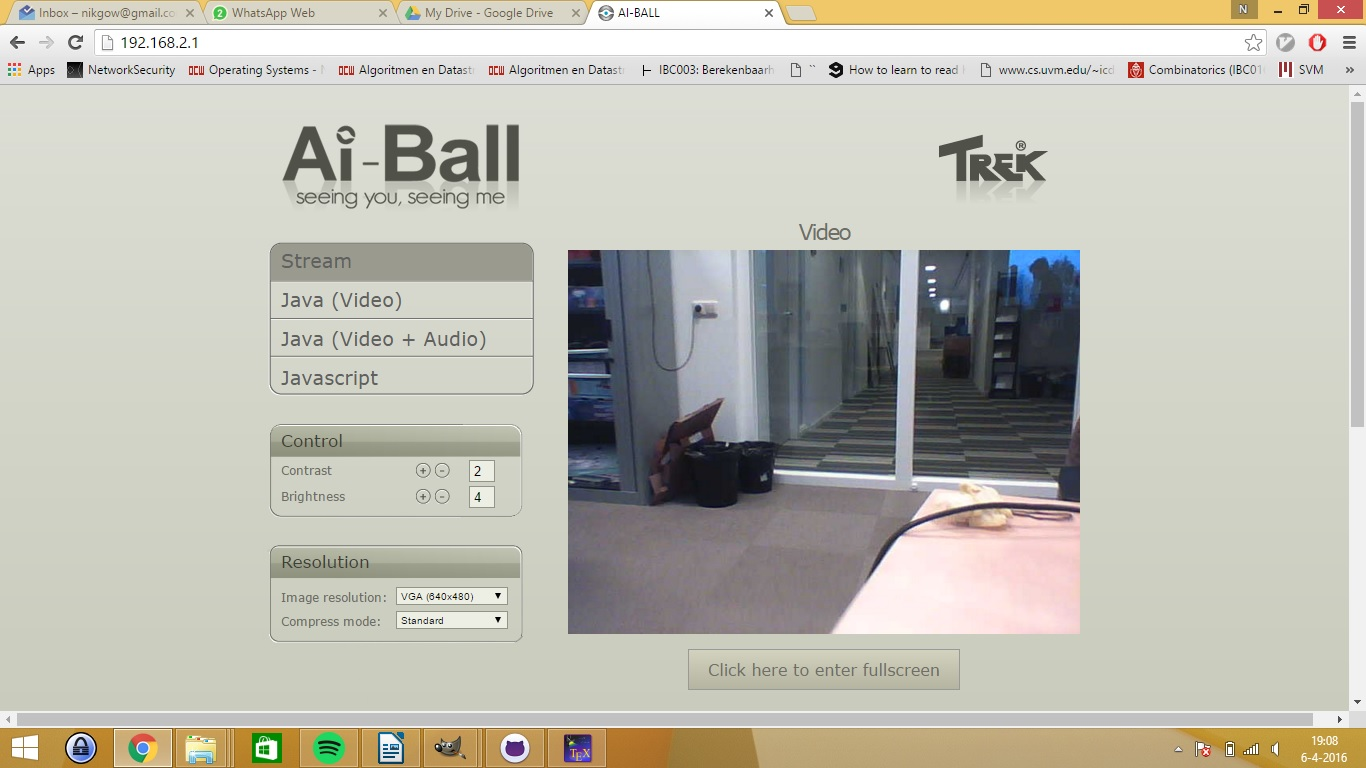
\includegraphics[width=0.7\linewidth]{trek_settings}
		\label{fig:trek_settings}
	\end{figure}
\end{enumerate}

\subsection{android app}
De app is zowel met als zonder Ai-ball te gebruiken. Met onderstaande methode kun je zowel met Wheelie als met Auto verbinden. Om de app te kunnen gebruiken is het nodig de bluetooth module op de robot te monteren. Om te kunnen zien waar de robot rijd, is het ook nodig de Ai-ball te monteren. Maar ook zonder Ai-ball is de app te gebruiken. In dat geval kun je stap 1 overslaan.

\begin{enumerate}
	\item Verbind je mobiel met de Ai ball. Dit doe je door de eerste 2 stappen onder het kopje "Ai ball" uit te voeren.
	\item Open de app.
	\item Zorg dat bluetooth aanstaat. Indien dit nog niet zo is als je de app opent, zal deze een pop-up geven met de vraag dit alsnog voor je te doen. 
	\item Zorg dat de robot aanstaat. 
	\item Zorg dat je je mobiel in de neutrale positie staat. Dit is de positie waarbij de robot stil staat. Dit doe je om te voorkomen dat als je de robot verbindt met de app, dat dan de robot er opeens vandoor gaat. Let op, de neutrale positie van Wheelie en Auto verschilt. 
	\begin{enumerate}
		\item De neutrale positie van Wheelie is: scherm in landscape mode, de telefoon verticaal omhoog en het scherm naar je toe gekeerd.
		\item De neutrale positie van Auto is: scherm in landscape mode, het scherm naar je toe gekeerd en de telefoon in een hoek van 45 graden van je af gedraaid. 
	\end{enumerate} 
	\item Verbind de app met de robot. Druk op de "Connect" knop bovenin de app. Hierna krijg je alle beschikbare bluetooth apparaten te zien. Selecteer het gewenste apparaat om ermee te verbinden.
	\begin{enumerate}
		\item De devicename van Wheelie is "WHEELIE".
		\item De devicename van Auto is "AUTO".
	\end{enumerate}
\end{enumerate}

\newpage
\begin{thebibliography}{9}
\bibitem{BLE_tutorial}
Townsend, K. (2015, 04 mei). Getting Started with the nRF8001 Bluefruit LE Breakout. 
Geraadpleegd van \url{https://learn.adafruit.com/getting-started-with-the-nrf8001-bluefruit-le-breakout/}

\bibitem{BLE_voorbeeldapp}
tdicola (2015, 06 oktober). BTLETest. Geraadpleegd van \url{https://github.com/tdicola/BTLETest/}

\bibitem{acc_tutorial}
zagGrad (2011, 10 januari). ADXL345 Quickstart Guide. Geraadpleegd van \url{https://www.sparkfun.com/tutorials/240}

\bibitem{BLE_specs}
KIWI electronics. (z.j.). 
BLUEFRUIT LE - BLUETOOTH LOW ENERGY (BLE 4.0) - NRF8001 BREAKOUT. Geraadpleegd van \url{https://www.kiwi-electronics.nl/bluefruit-le-bluetooth-low-energy-ble-4-0-nRF8001-breakout}

\bibitem{UNO_specs}
ARDUINO. (z.j). Arduino UNO \& Genuino UNO. Geraadpleegd van \url{https://www.arduino.cc/en/Main/ArduinoBoardUno}

\bibitem{acc_specs}
SparkFun. (z.j). SparkFun Triple Axis Accelerometer Breakout - ADXL345. Geraadpleegd van \url{https://www.sparkfun.com/products/9836}

\bibitem{DIY_specs}
DX. (z.j). DIY Intelligent Tortoise Smart Wheel Robot Module-Black. Geraadpleegd van 
\url{http://www.dx.com/p/diy-intelligent-tortoise-smart-wheel-robot-module-173668?tc=EUR&gclid=CI7qtbm5p78CFa_KtAodTSgAVA#.VvvjLeKLTIW}

\bibitem{DIY_auto}
DX. (z.j). Bluetooth Controlled Robot Car Kits for Arduino. Geraadpleegd van
\url{http://www.dx.com/p/arduino-compatible-bluetooth-controlled-robot-car-kits-146418#.VwTq0PmLTIV}

\bibitem{DIY_auto_hl}
Anonymous. (z.j). Arduino Bluetooth utility vehicle manual. Geraadpleegd van
\url{http://m5.img.dxcdn.com/CDDriver/CD/sku.146418.docx}

\bibitem{camera_specs}
AI-Ball. (z.j). What is an AI-ball? Geraadpleegd van
\url{http://www.thumbdrive.com/aiball/intro.html}

\bibitem{Balancing_robot}
Dorweiler, J. (2012, 27 mei). Balancing Robot. Geraadpleeg van
\url{http://www.transistor.io/balancing-robot.html}

\bibitem{voorbeeld2}
Short, J. (z.j). How to Build a Self-Balancing Autonomous Arduino Bot. Geraadpleegd van 
\url{http://makezine.com/projects/arduroller-self-balancing-robot/}

\bibitem{ARDUINO_getting started}
ARDUINO. (z.j). Getting Started with Arduino. Geraadpleegd van \url{https://www.arduino.cc/en/Guide/HomePage}

\bibitem{nrf_ua}
NordicSemiconductor. (2015, 6 oktober) Android-nRF-UART. Geraadpleegd van 
\url{https://github.com/NordicSemiconductor/Android-nRF-UART}

\end{thebibliography}

\end{document}
